\section{Results}

Table \ref{tab:measured_growth_parameters} shows the measured growth parameters: plant height\index{growth parameter!plant height}, stem circumference\index{growth parameter!stem circumference}, and number of internodes\index{growth parameter!number of internodes} at the end of the experiment after \num[mode=text]{46} days for both the UV and the control groups. Note that plant number \num[mode=text]{4} (control) died.

Figures \ref{fig:plants_uv_2024-05-13} and \ref{fig:plants_ctrl_2024-05-13} show the plants treated with UV light and the plants of the control group, respectively, on May 13 when the plants were transplanted into \qty[mode=text]{15}{\L} containers. Figures \ref{fig:plants_uv_2024-06-17} and \ref{fig:plants_ctrl_2024-06-17} show the plants of the UV and control groups, respectively, on June 17, including their experimental setups. Figure \ref{fig:plant_all_2024-06-17} shows all plants together on June 17.

\begin{table}[htbp]
    \caption[Measured growth parameters of the cannabis plants]{Measured growth parameters of the cannabis plants on June 17, \num[mode=text]{46} days after planting the seeds.}
    \label{tab:measured_growth_parameters}
    \begin{tabularx}{\linewidth}{llcccc}
        \toprule
        \textbf{Group} & \textbf{Cultivar} & \textbf{Plant \#} & \textbf{Height (\unit[mode=text]{\cm})} & \textbf{Stem cir. (\unit[mode=text]{\cm})} & \textbf{\#{}Internodes} \\
        \midrule
        \multirow{6}{*}{UV} & Skywalker Haze & 1 & 49 & 4.3 & 11 \\
        & \multirow[t]{5}{*}{Frisian Dew} & 3 & 59 & 5.5 & 12 \\
        & & 5 & 56 & 5.5 & 12 \\
        & & 7 & 54 & 5.1 & 11 \\
        & & 9 & 56 & 5.5 & 12 \\
        & & 11 & 52 & 4.7 & 12 \\
        \midrule
        \multirow{6}{*}{Control} & Skywalker Haze & 2 & 49 & 5.0 & 12 \\
        & \multirow[t]{5}{*}{Frisian Dew} & 4 & - & - & - \\
        & & 6 & 49 & 6.0 & 13 \\
        & & 8 & 60 & 5.5 & 12 \\
        & & 10 & 69 & 5.0 & 12 \\
        & & 12 & 52 & 5.8 & 12 \\
        \bottomrule
    \end{tabularx}
\end{table}

\subsection{Statistical analysis}

\subsubsection{Initial hypothesis}

The initial hypothesis of this experiment was: "Exposure to UV-A light at controlled low intensities enhances the germination rate and seedling development of Cannabis seeds by inducing protective and growth-promoting biochemical responses."

\subsubsection{Analysis procedure}

For the statistical analysis, we focused only on the Frisian Dew cultivar since there is only one Skywalker Haze plant in each group, which is insufficient for deriving statistical conclusions. The following statistical analyses were conducted:
\begin{enumerate}
    \item \emph{Descriptive statistics:} Calculation of mean and standard deviation for each growth parameter (plant height, stem circumference, and number of internodes) in both groups.
    \item \emph{Welch's t-test\index{statistics!Welch's t-test}:} Comparison of means between the UV and control groups for each growth parameter to determine if there were significant differences.
\end{enumerate}

\subsubsection{Descriptive statistics}

Table \ref{tab:descriptive_statistics} provides the mean\index{statistics!mean} and standard deviation\index{statistics!standard deviation} for the growth parameters of the Frisian Dew cultivar in both the UV and control groups. These statistics are essential for understanding the variability and central tendency of the measured growth parameters within each group.

\begin{table}[htbp]
    \caption[Mean and standard deviation of growth parameters]{Mean and standard deviation of growth parameters for Frisian Dew cultivar}
    \label{tab:descriptive_statistics}
    \begin{tabularx}{\linewidth}{l|XX|XX|XX}
        \toprule
        \textbf{Group} & \multicolumn{2}{l|}{\textbf{Height (\unit[mode=text]{\cm})}} & \multicolumn{2}{l|}{\textbf{Stem cir. (\unit[mode=text]{\cm})}} & \multicolumn{2}{l}{\textbf{\# Internodes}} \\
        & \textbf{Mean} & \textbf{SD} & \textbf{Mean} & \textbf{SD} & \textbf{Mean} & \textbf{SD} \\
        \midrule
        UV & \num[mode=text]{55} & \num[mode=text]{2.6} & \num[mode=text]{5.3} & \num[mode=text]{0.36} & \num[mode=text]{12} & \num[mode=text]{0.45} \\
        Control & \num[mode=text]{58} & \num[mode=text]{9.0} & \num[mode=text]{5.6} & \num[mode=text]{0.43} & \num[mode=text]{12} & \num[mode=text]{0.50} \\
        \bottomrule
    \end{tabularx}
\end{table}

\subsubsection{T-test analysis}

To compare the growth parameters between the UV and control groups for the Frisian Dew cultivar, an independent samples t-test (Welch's t-test\index{statistics!Welch's t-test}) was conducted. This type of t-test is used to determine if there is a statistically significant difference between the means of two groups. The test assumes that the two groups are independent and that the data are approximately normally distributed, without assuming equal variances between groups.

The results of the t-tests for plant height, stem circumference, and number of internodes are presented in Table \ref{tab:ttest_results}. These results indicate no significant differences between the UV and control groups for any of the measured growth parameters, suggesting that UV light exposure did not significantly influence these parameters under the conditions of this experiment.

Therefore, these findings do not support the initial hypothesis that UV light enhances germination rate and seedling development through protective and growth-promoting biochemical responses.

\begin{table}[htbp]
    \caption{Welch's t-test results for growth parameters}
    \label{tab:ttest_results}
    \begin{tabularx}{\linewidth}{lcc}
        \toprule
        \textbf{Parameter} & \textbf{t-value} & \textbf{p-value} \\
        \midrule
        Plant height & \num[mode=text]{-0.45} & \num[mode=text]{0.68} \\
        Stem cir. & \num[mode=text]{-1.17} & \num[mode=text]{0.29} \\
        \# Internodes & \num[mode=text]{-1.41} & \num[mode=text]{0.21} \\
        \bottomrule
    \end{tabularx}
\end{table}

\begin{figure}[htbp]
    \begin{subfigure}[t]{.19\textwidth}
        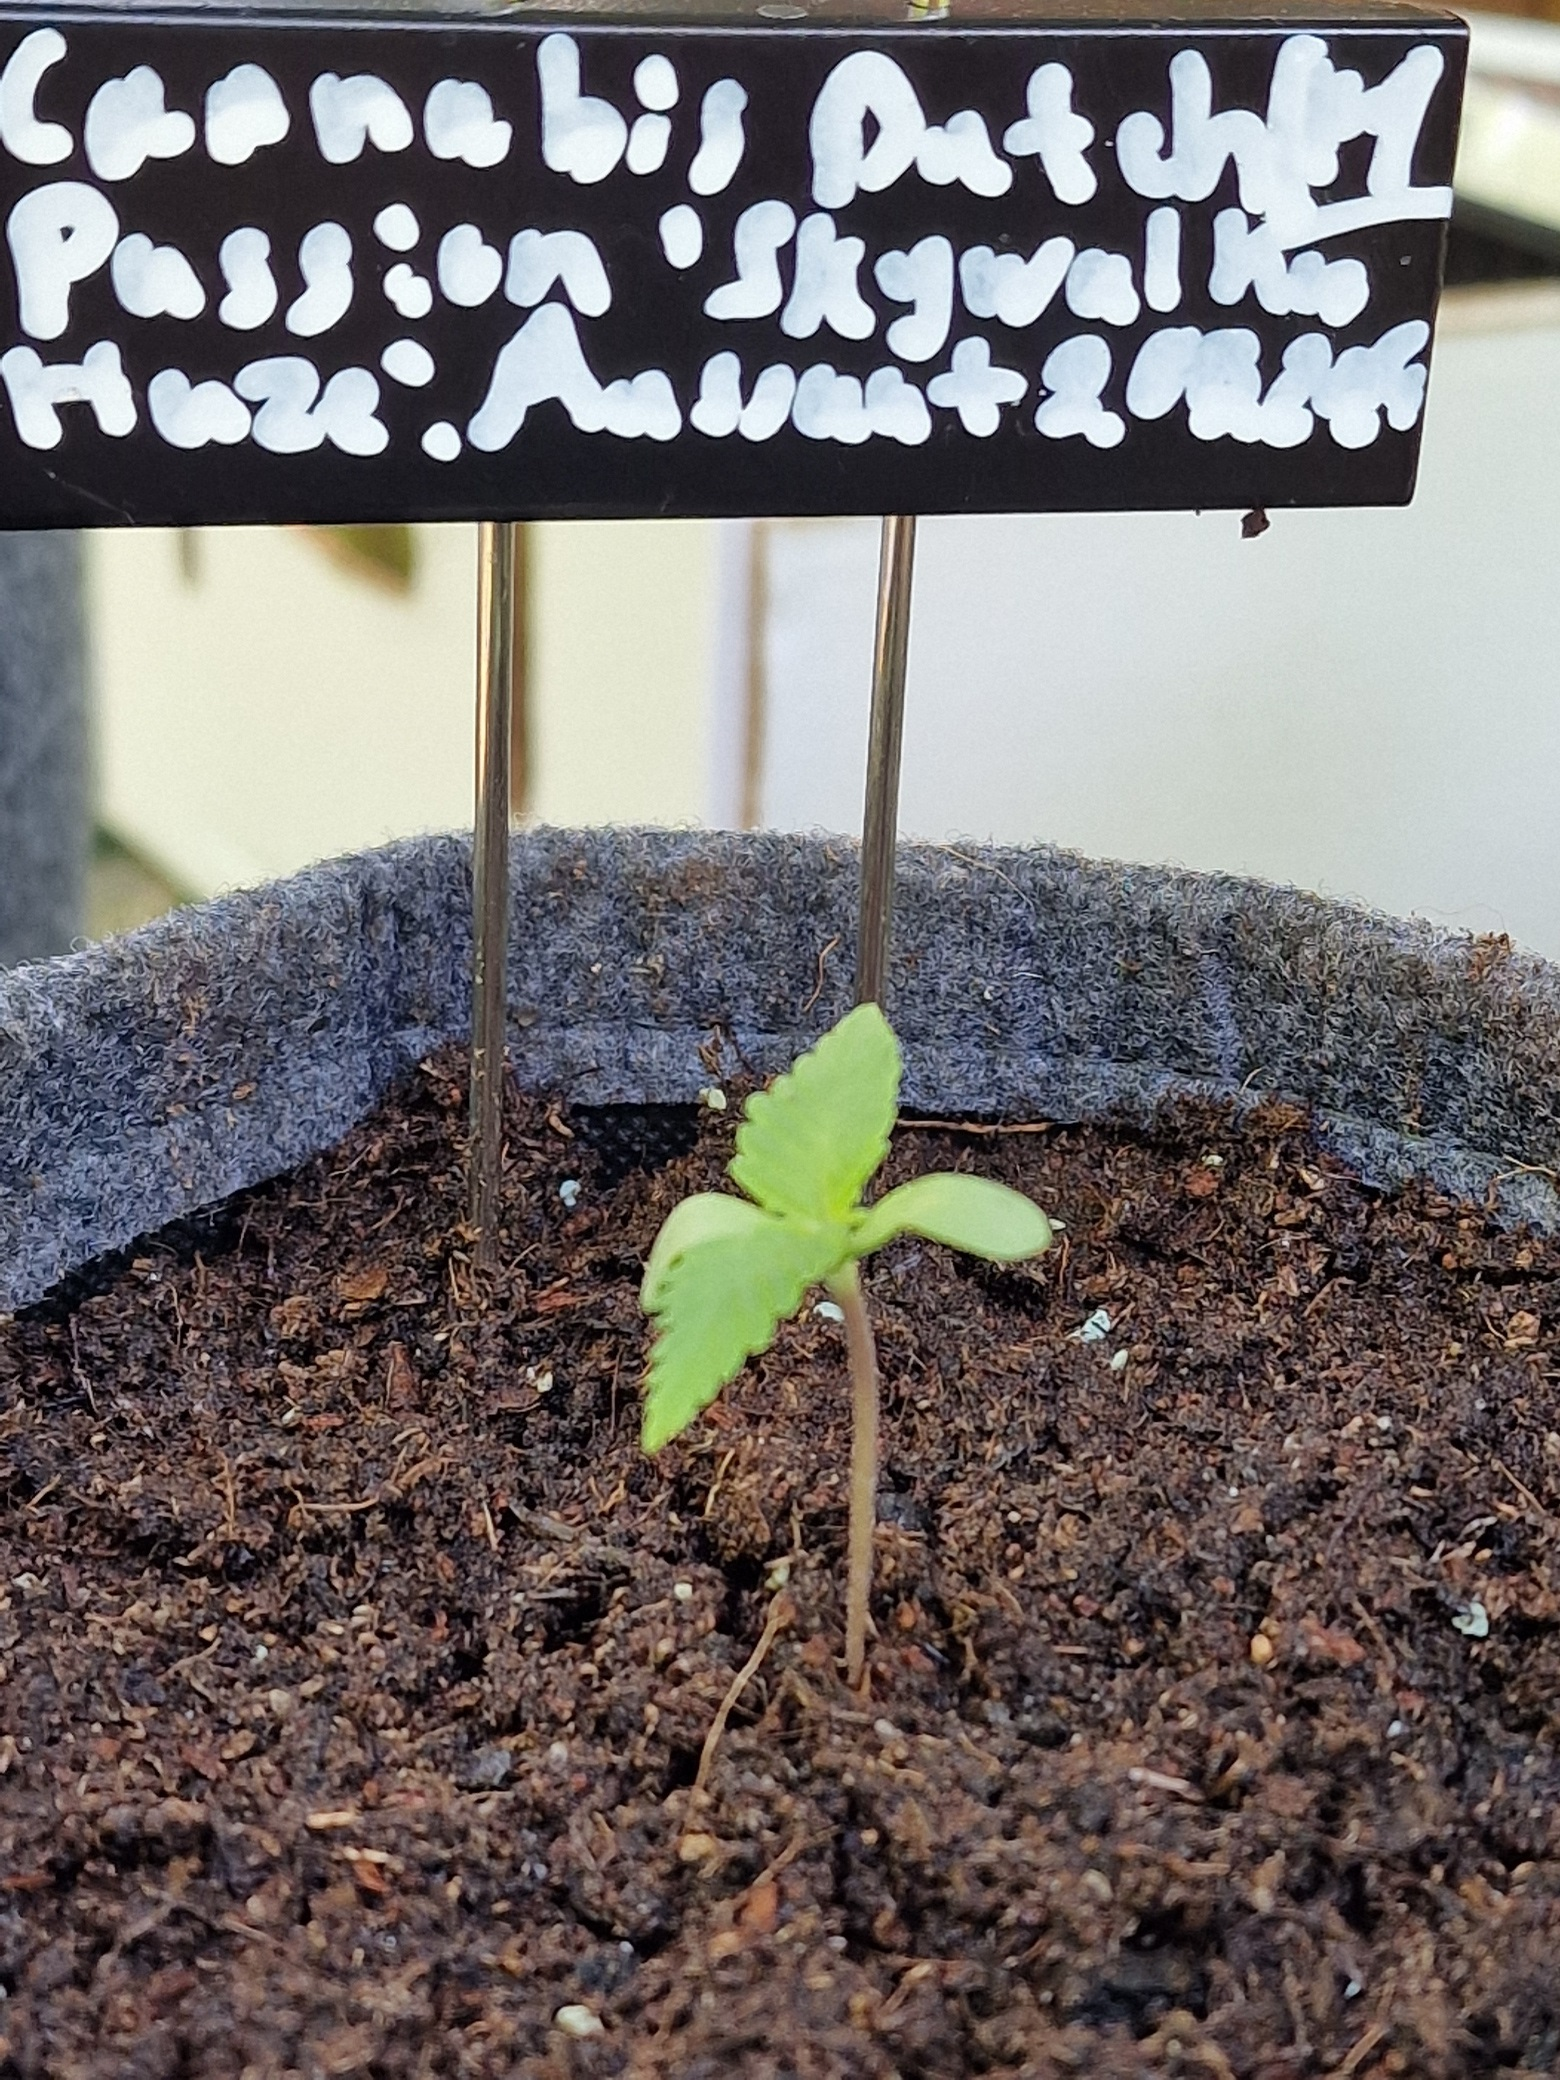
\includegraphics[width=\linewidth]{plant_01_2024-05-13}
        \caption{Plant \# 1}
        \label{fig:plant_01_2024-05-13}
    \end{subfigure}
    \begin{subfigure}[t]{.19\textwidth}
        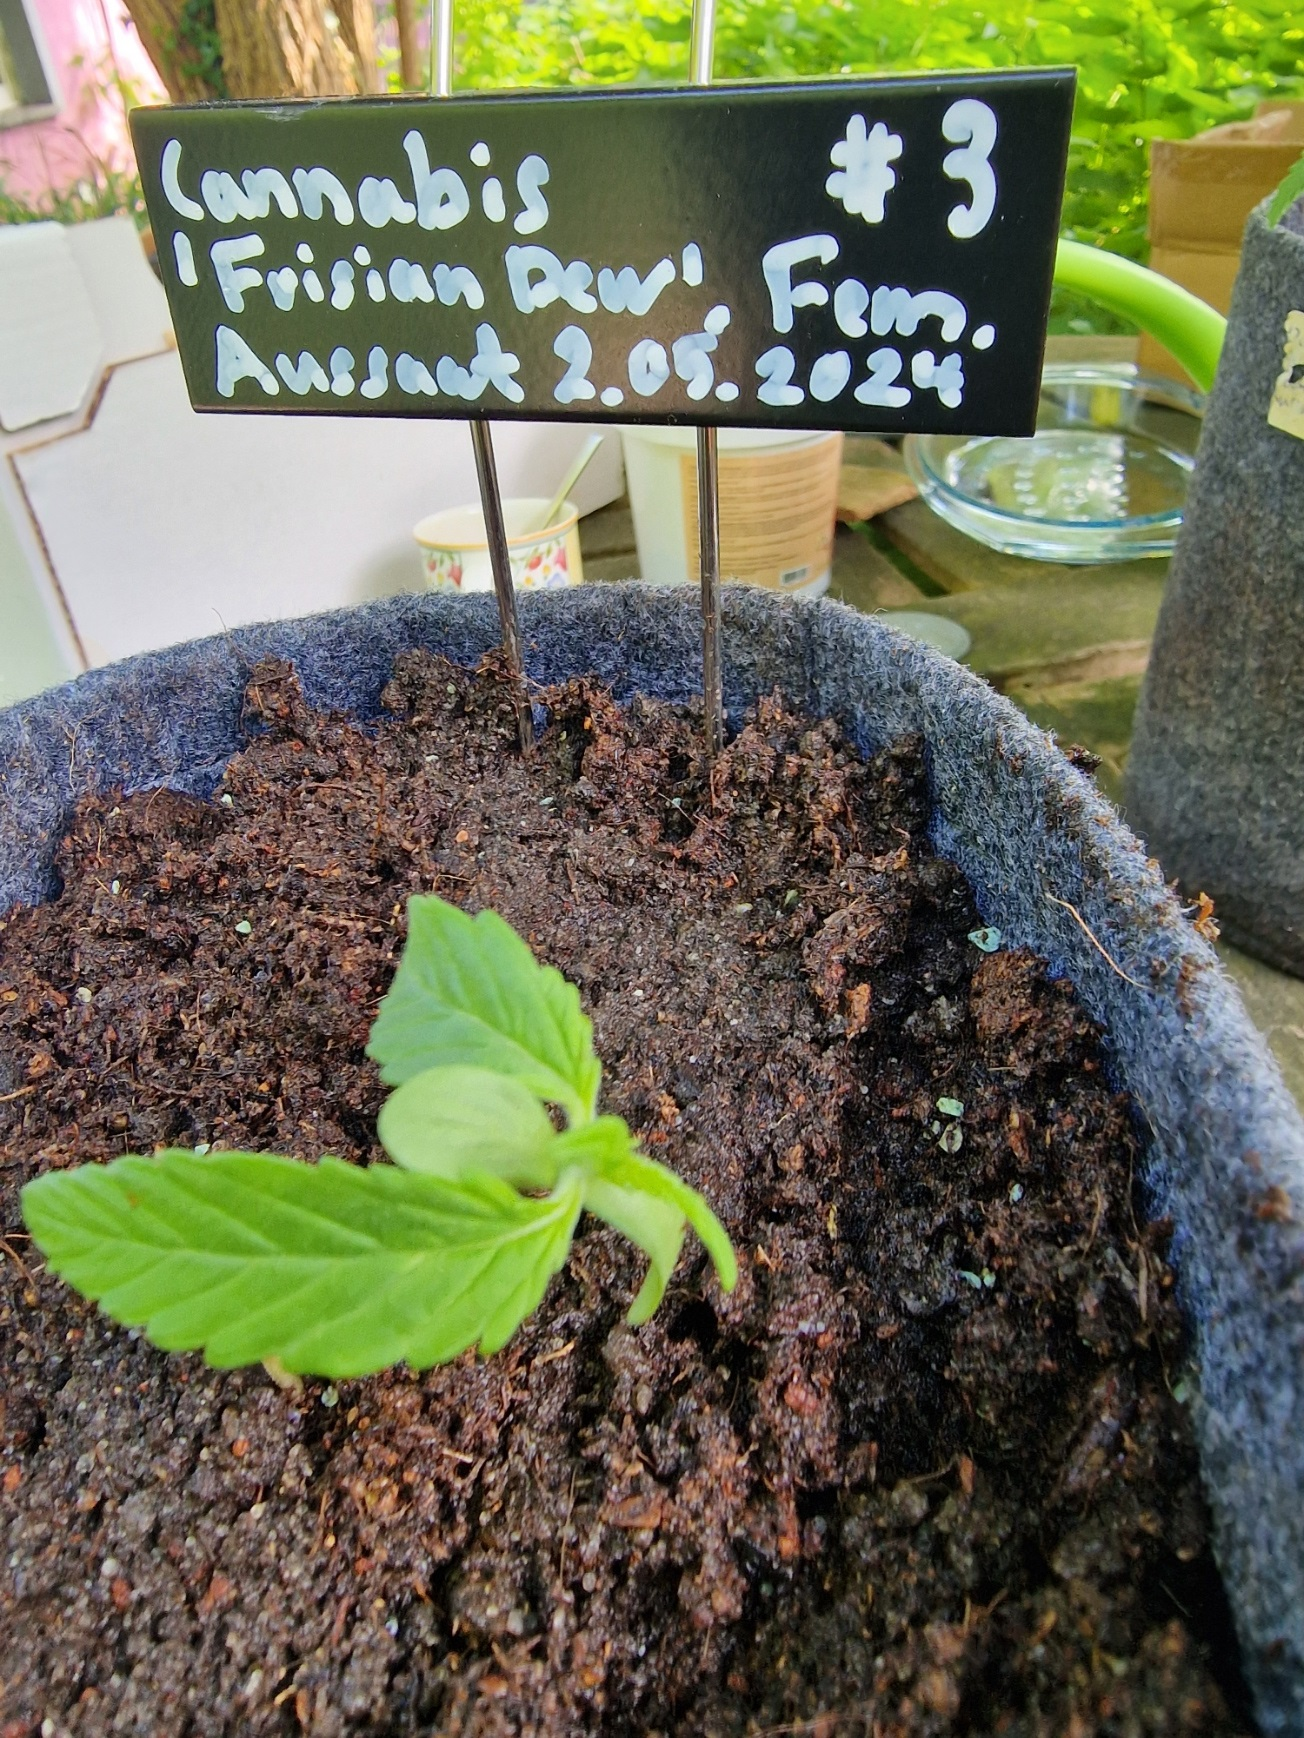
\includegraphics[width=\linewidth]{plant_03_2024-05-13}
        \caption{Plant \# 3}
        \label{fig:plant_03_2024-05-13}
    \end{subfigure}
    \begin{subfigure}[t]{.19\textwidth}
        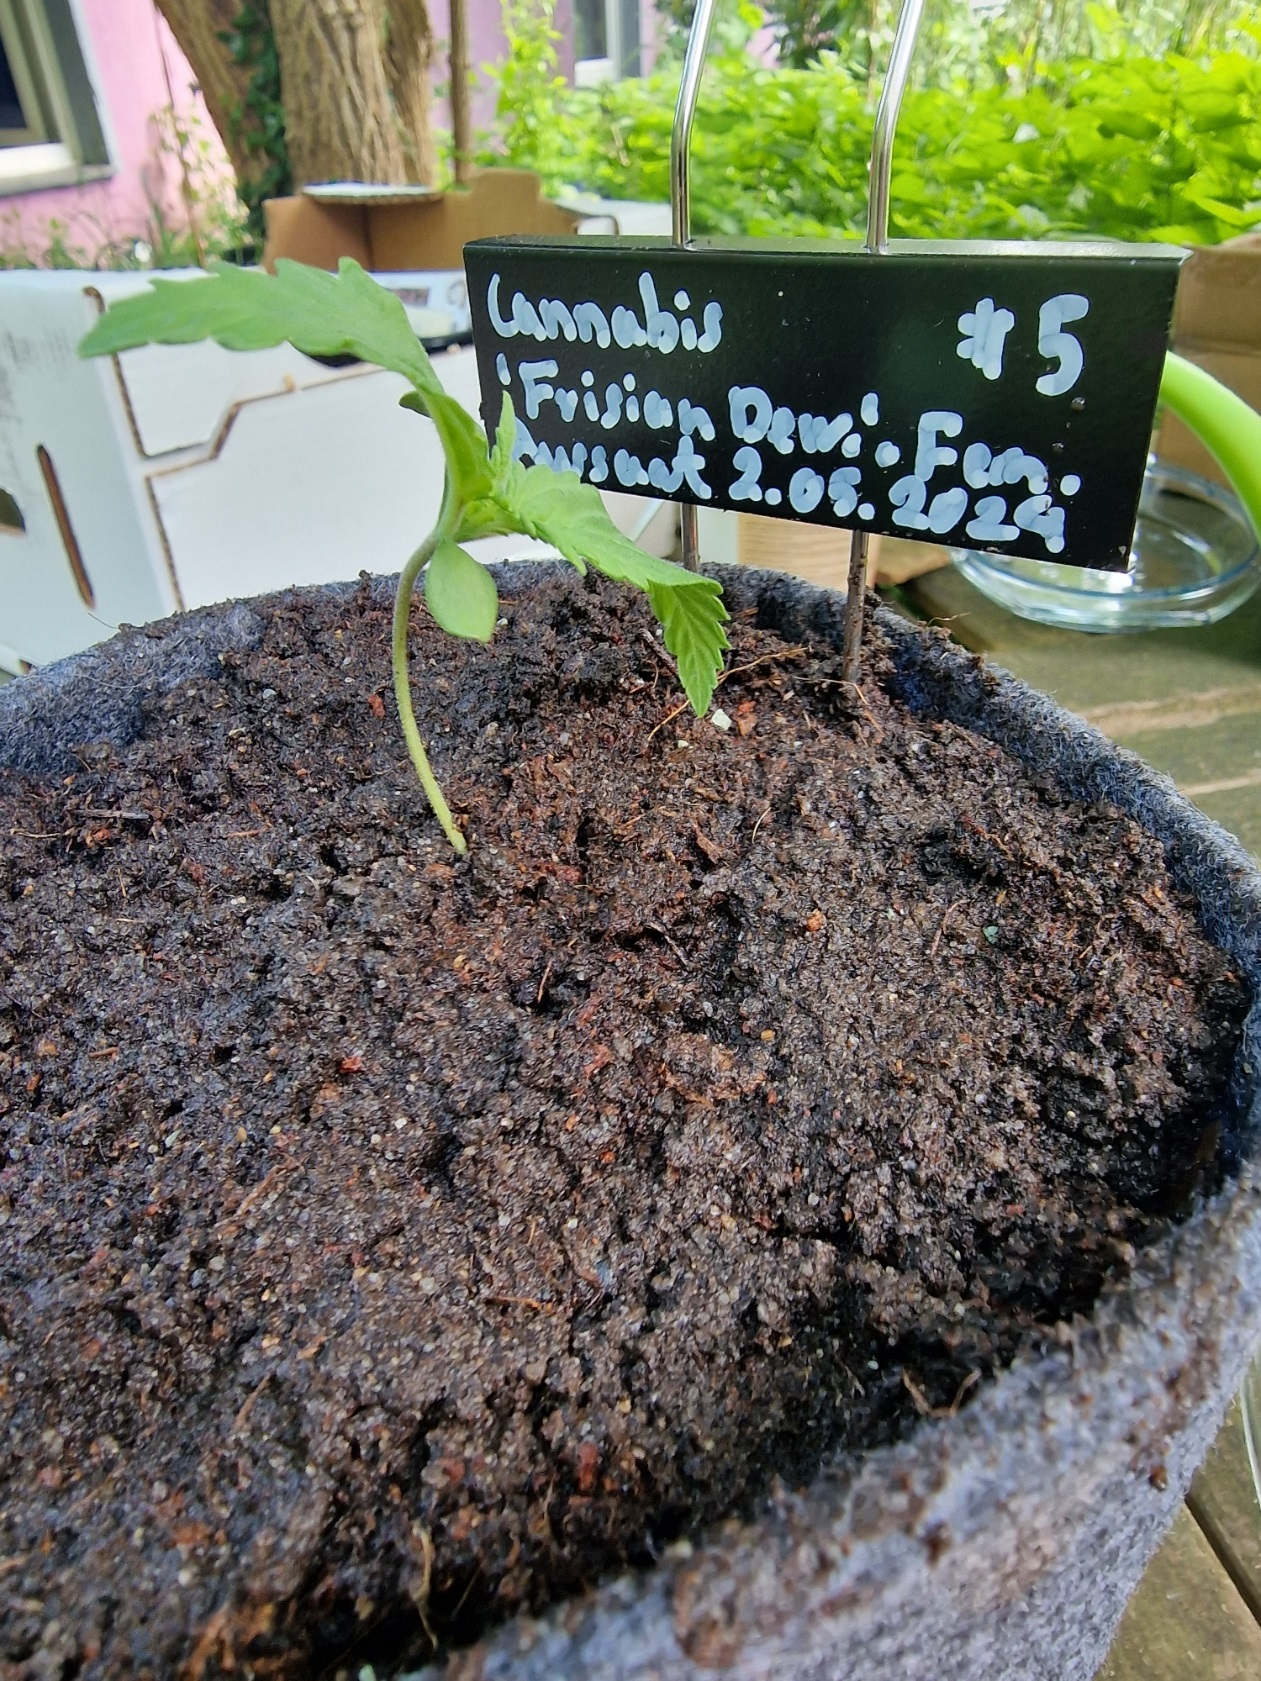
\includegraphics[width=\linewidth]{plant_05_2024-05-13}
        \caption{Plant \# 5}
        \label{fig:plant_05_2024-05-13}
    \end{subfigure}
    \begin{subfigure}[t]{.19\textwidth}
        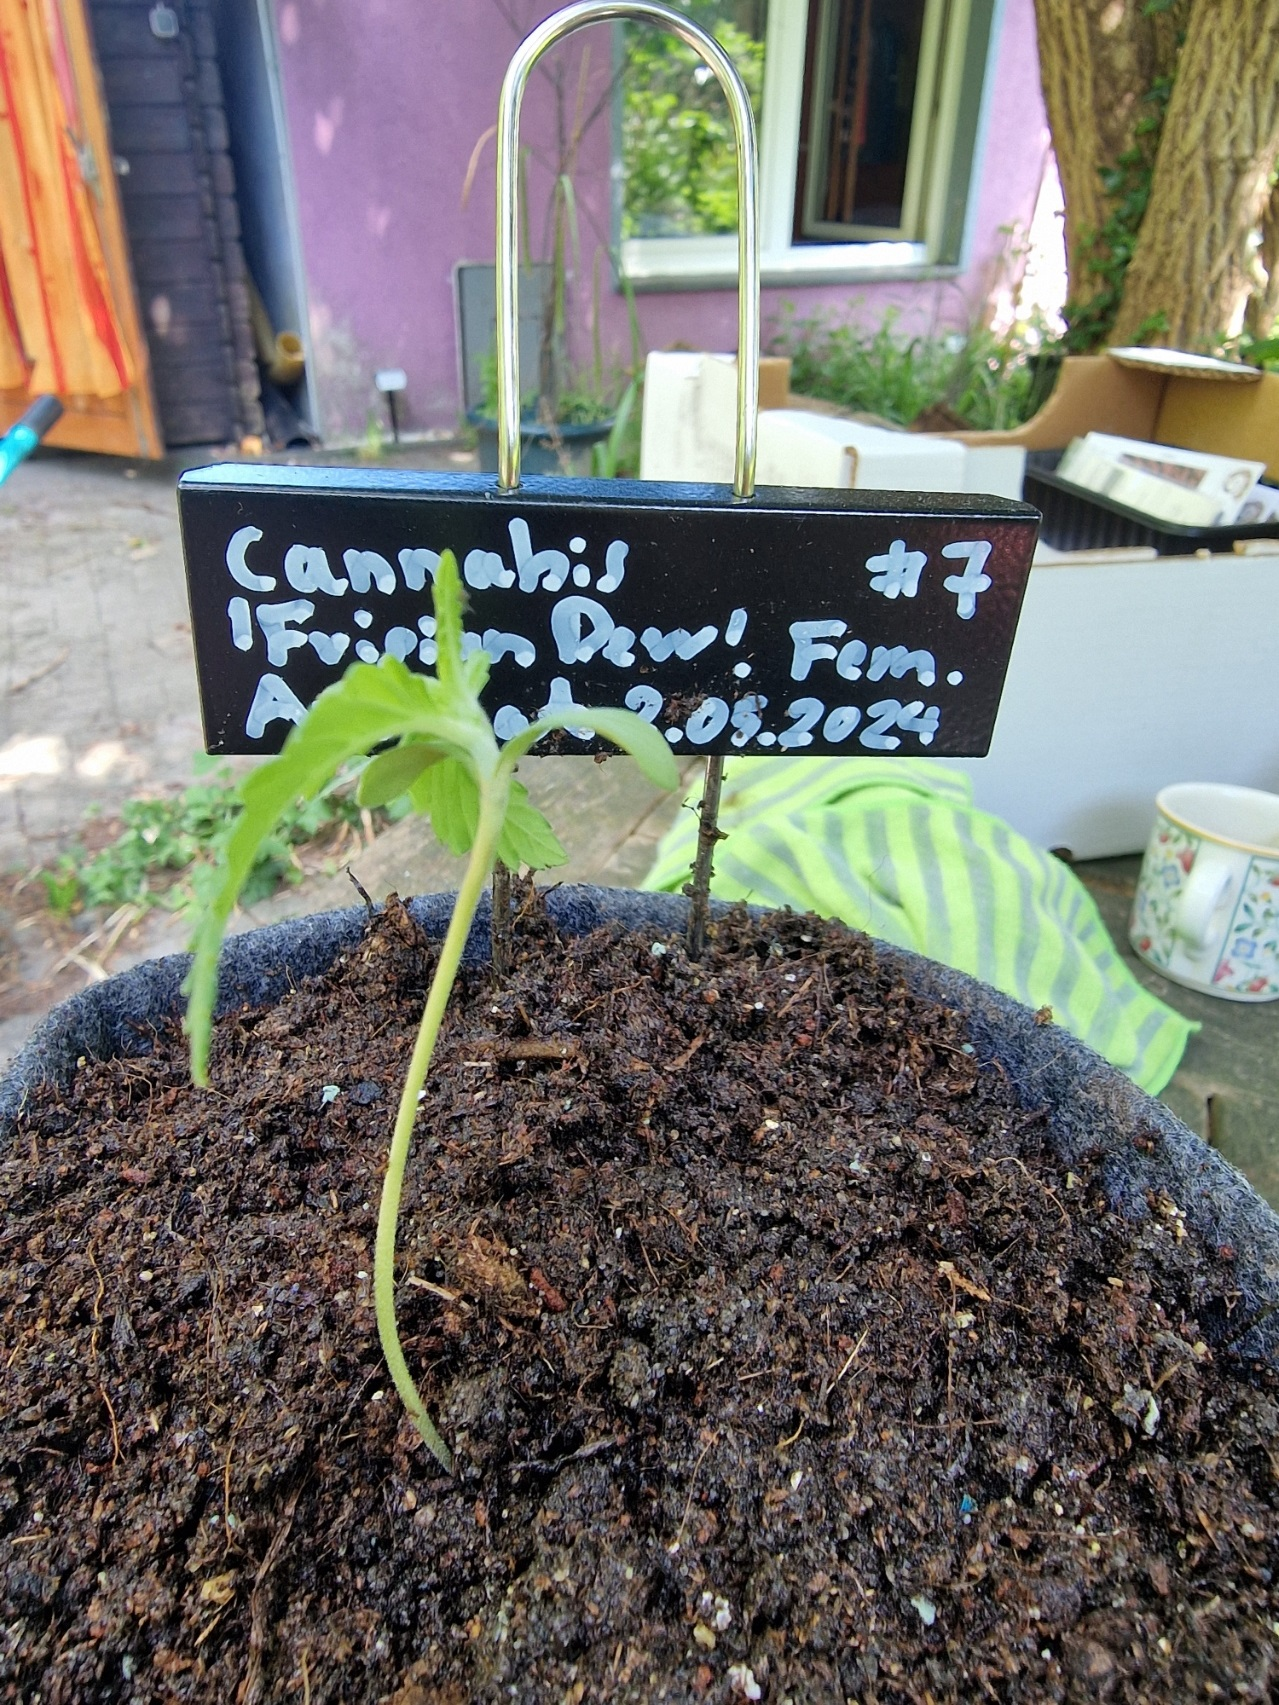
\includegraphics[width=\linewidth]{plant_07_2024-05-13}
        \caption{Plant \# 7}
        \label{fig:plant_07_2024-05-13}
    \end{subfigure}
    \begin{subfigure}[t]{.19\textwidth}
        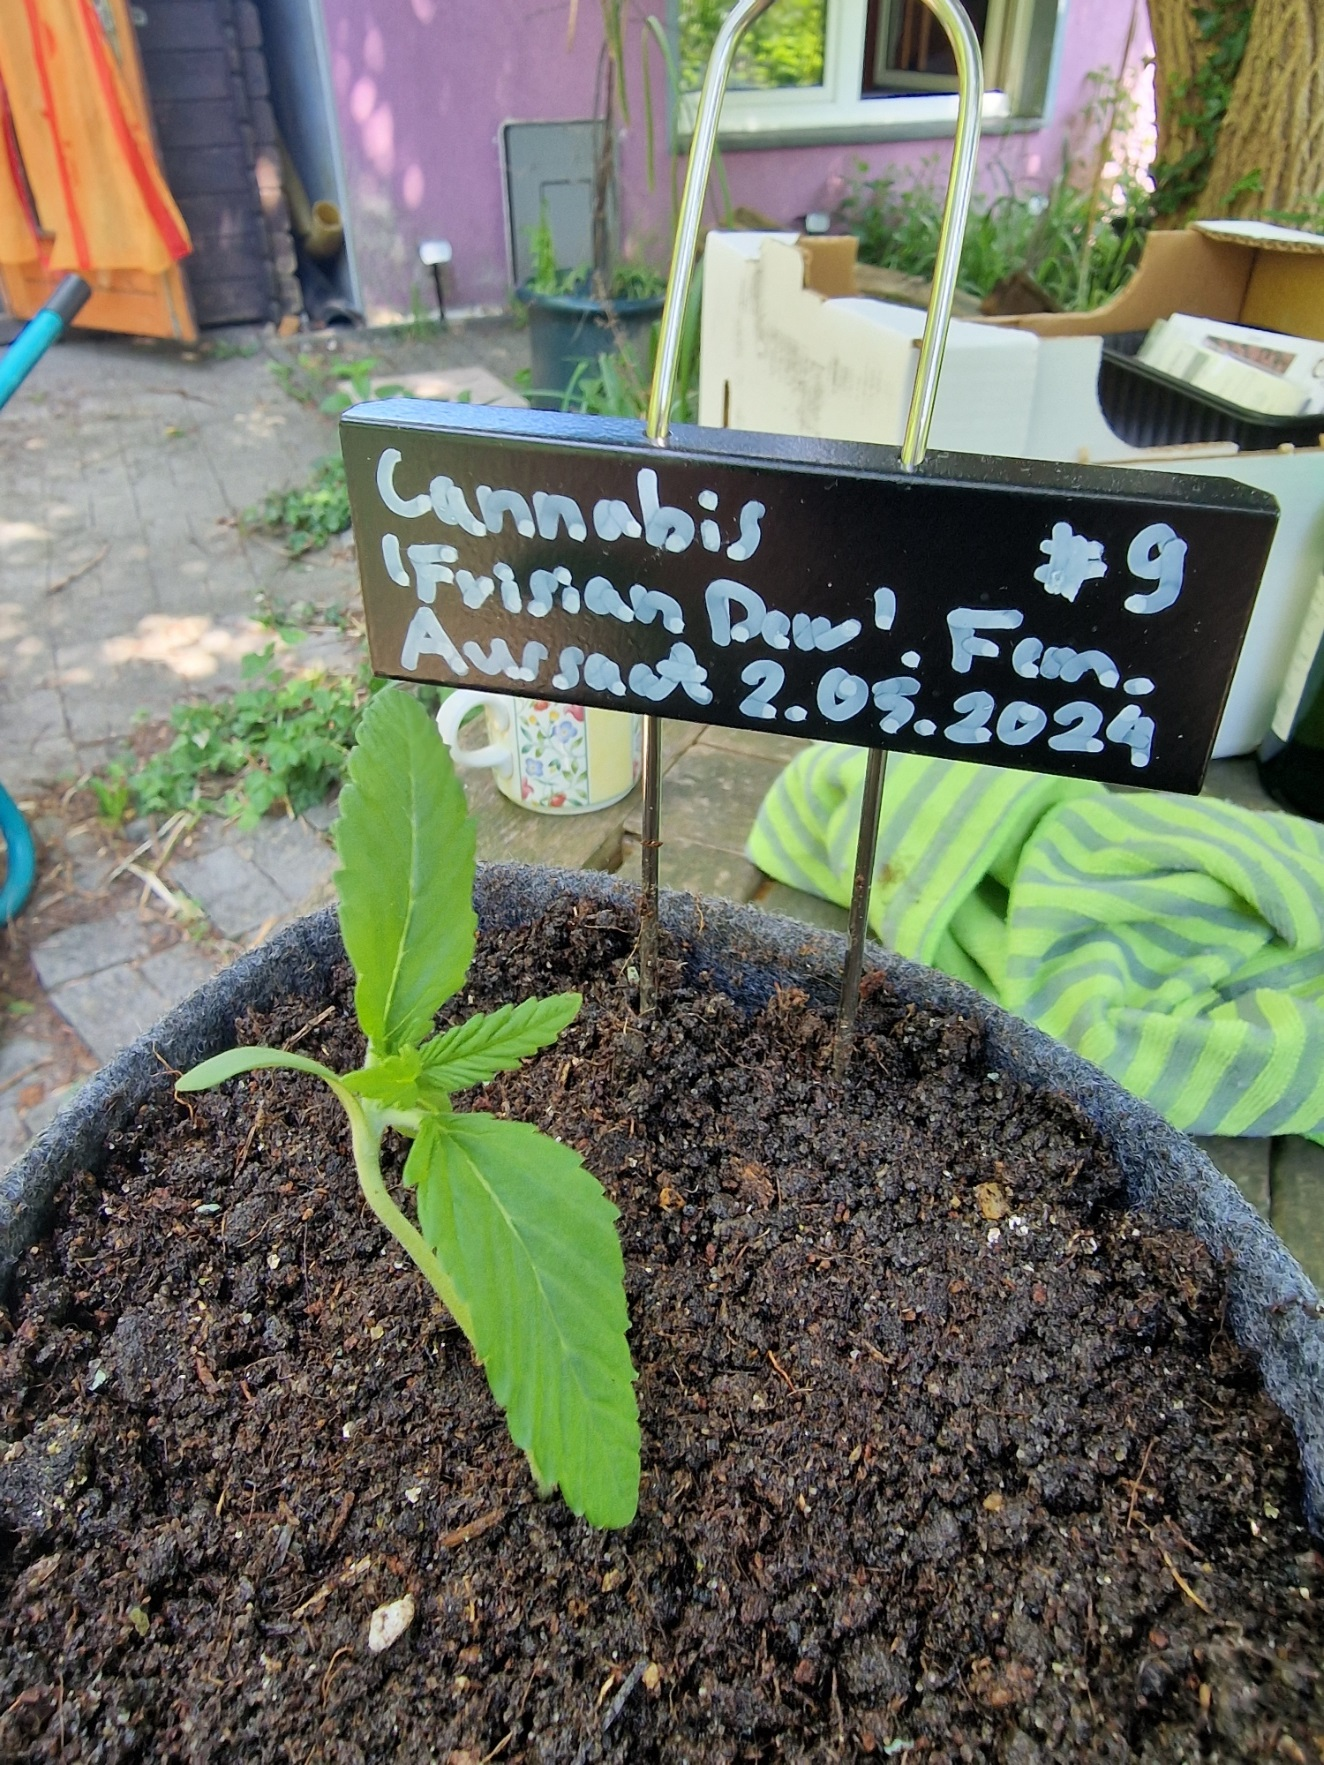
\includegraphics[width=\linewidth]{plant_09_2024-05-13}
        \caption{Plant \# 9}
        \label{fig:plant_09_2024-05-13}
    \end{subfigure}
    \caption[Plants of the UV group on May 13]{The plants treated with UV light on May 13}
    \label{fig:plants_uv_2024-05-13}
\end{figure}

\begin{figure}[htbp]
    \begin{subfigure}[t]{.19\textwidth}
        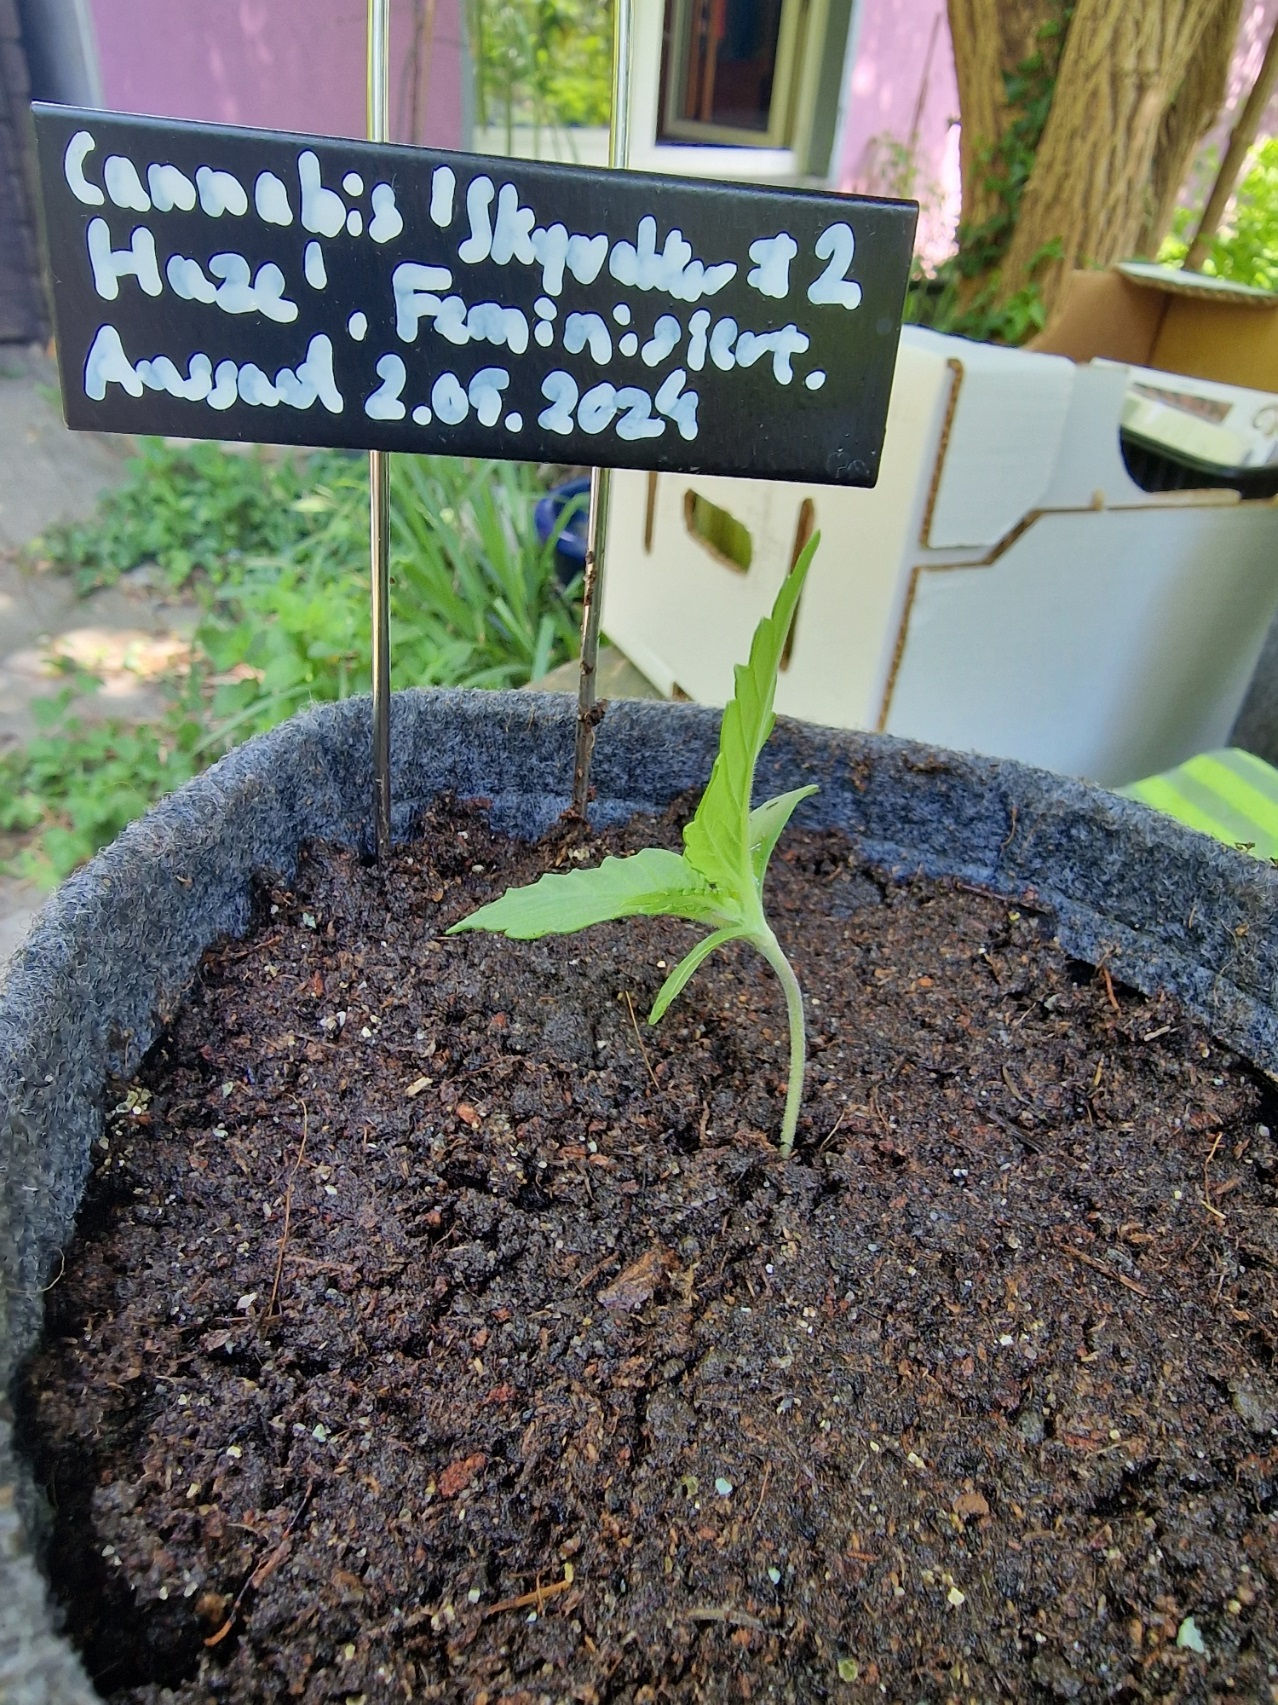
\includegraphics[width=\linewidth]{plant_02_2024-05-13}
        \caption{Plant \# 2}
        \label{fig:plant_02_2024-05-13}
    \end{subfigure}
    \begin{subfigure}[t]{.19\textwidth}
        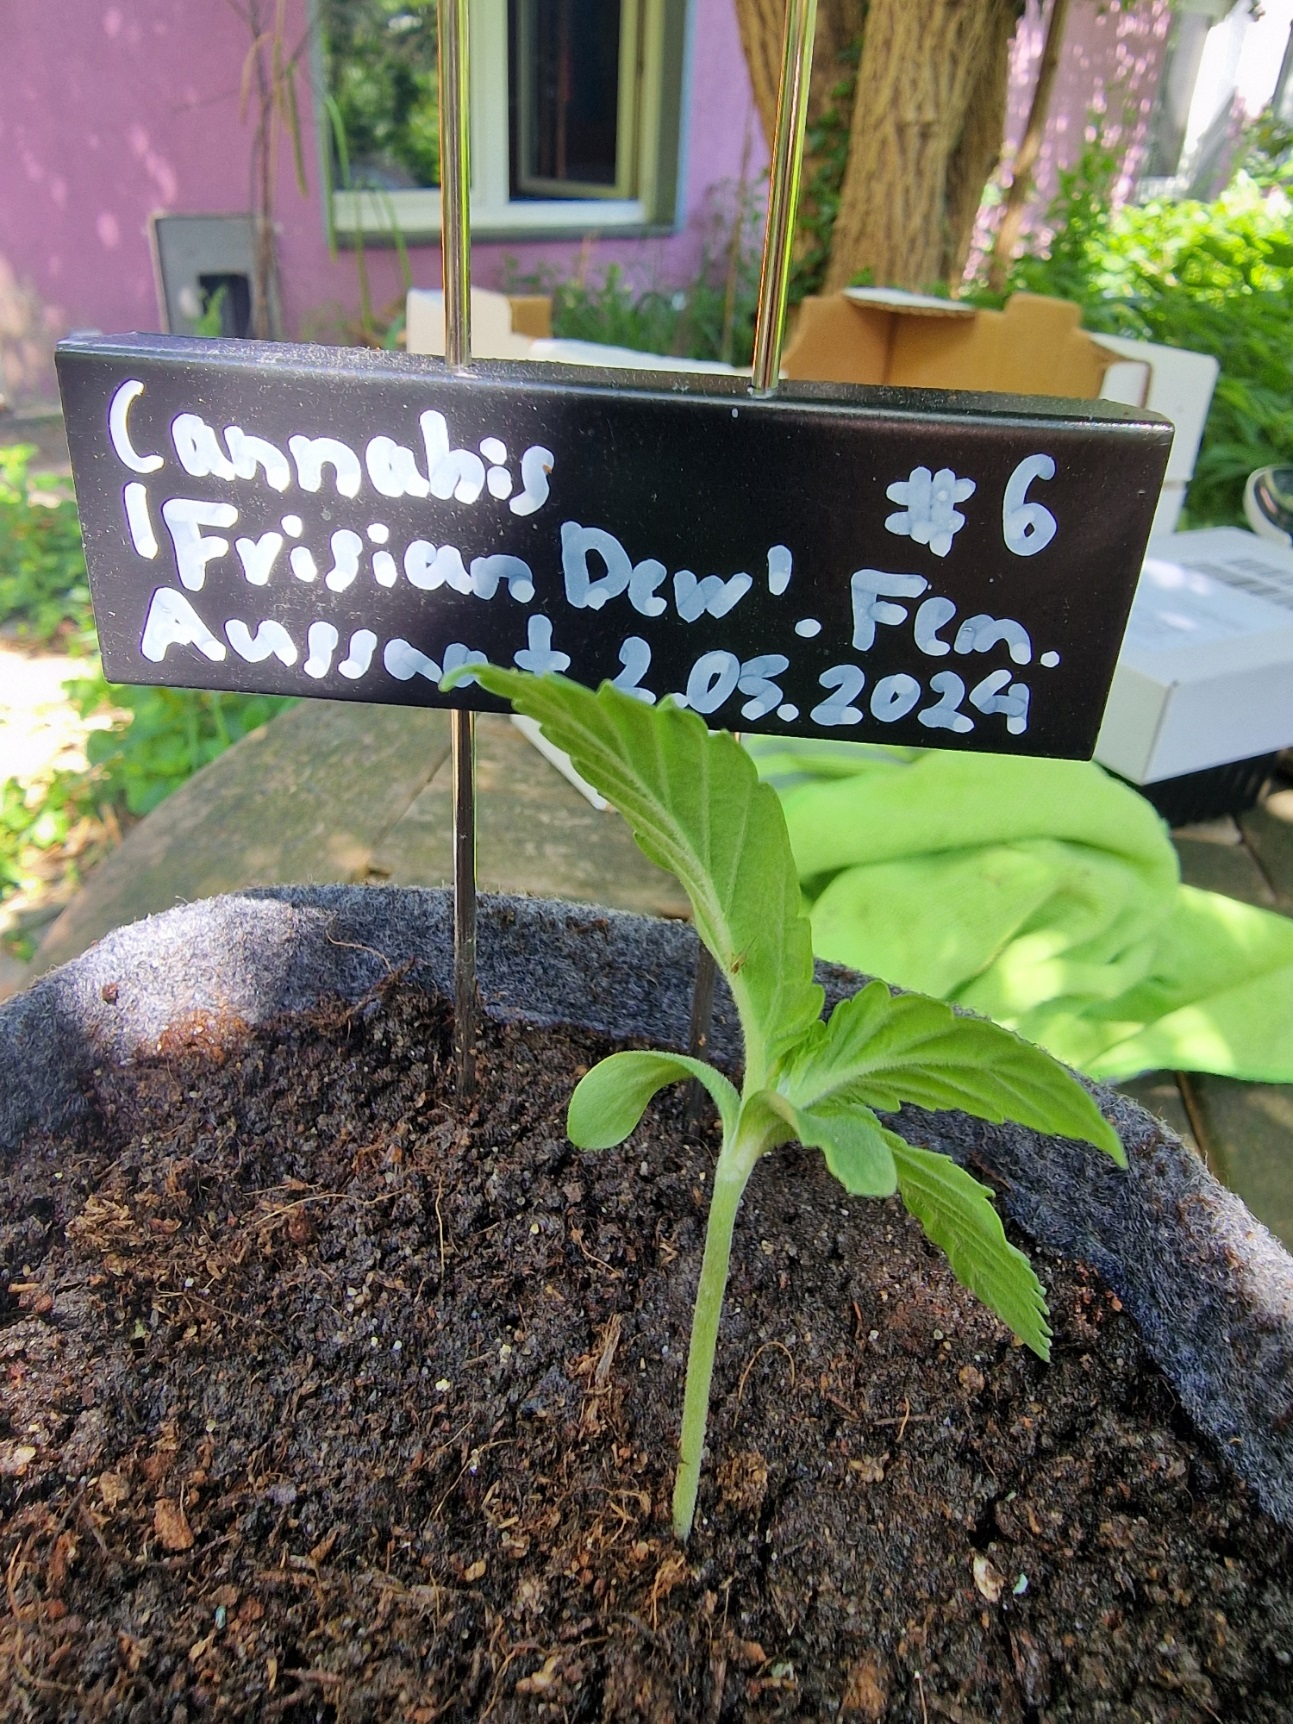
\includegraphics[width=\linewidth]{plant_06_2024-05-13}
        \caption{Plant \# 6}
        \label{fig:plant_06_2024-05-13}
    \end{subfigure}
    \begin{subfigure}[t]{.19\textwidth}
        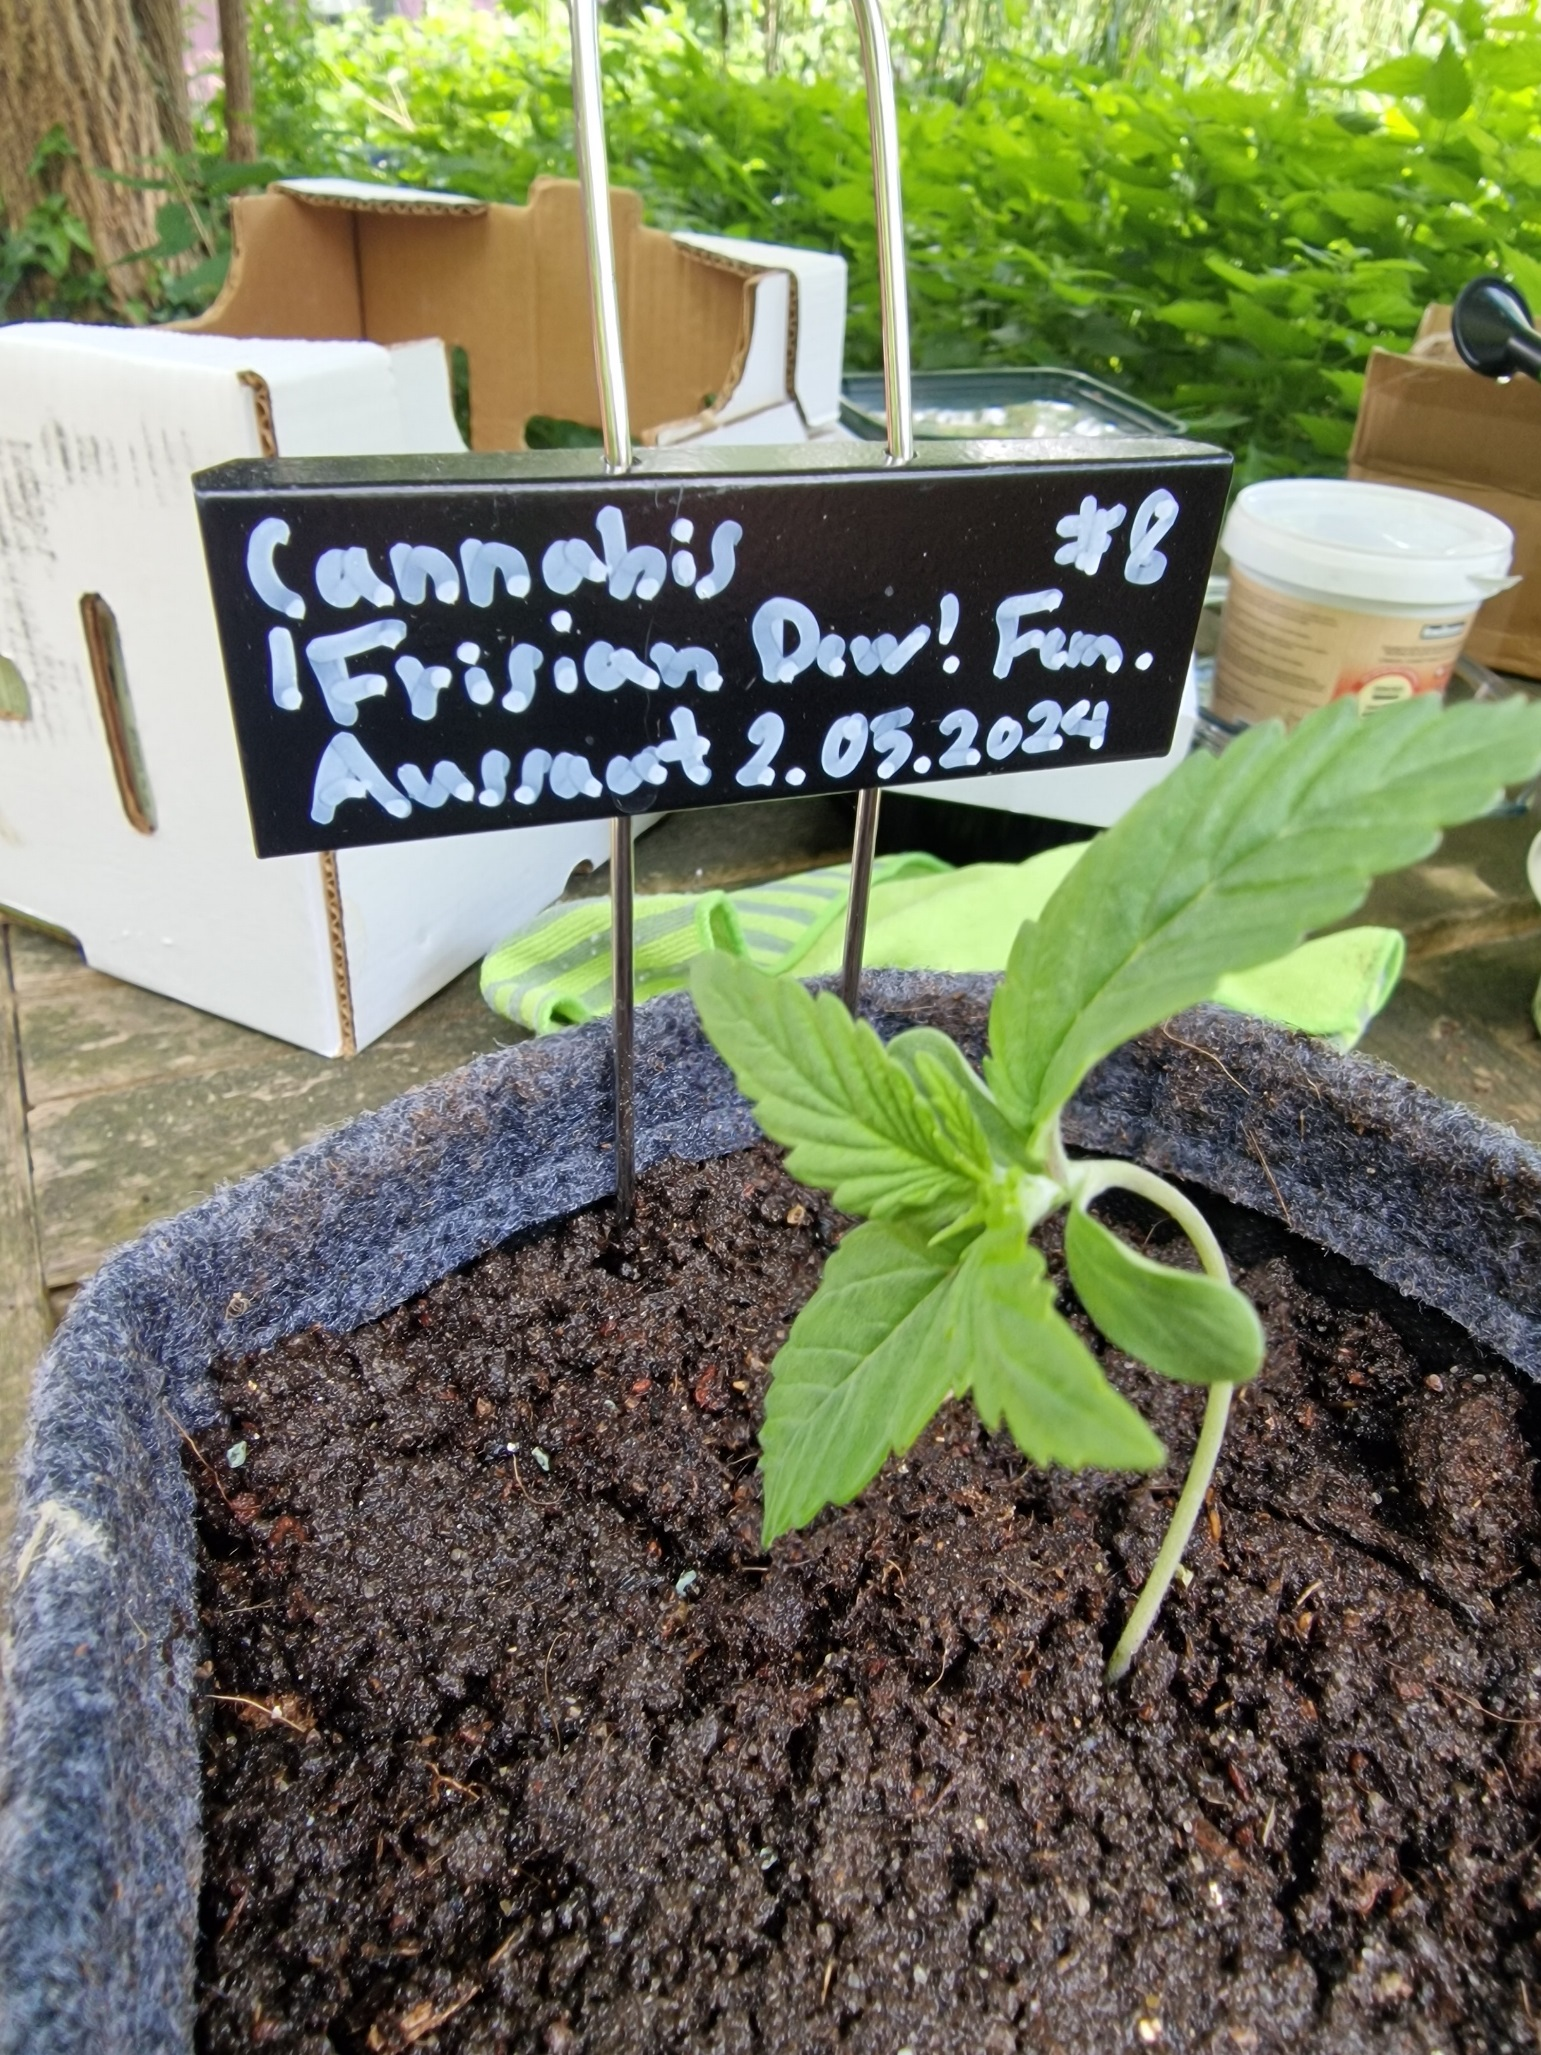
\includegraphics[width=\linewidth]{plant_08_2024-05-13}
        \caption{Plant \# 8}
        \label{fig:plant_08_2024-05-13}
    \end{subfigure}
    \begin{subfigure}[t]{.19\textwidth}
        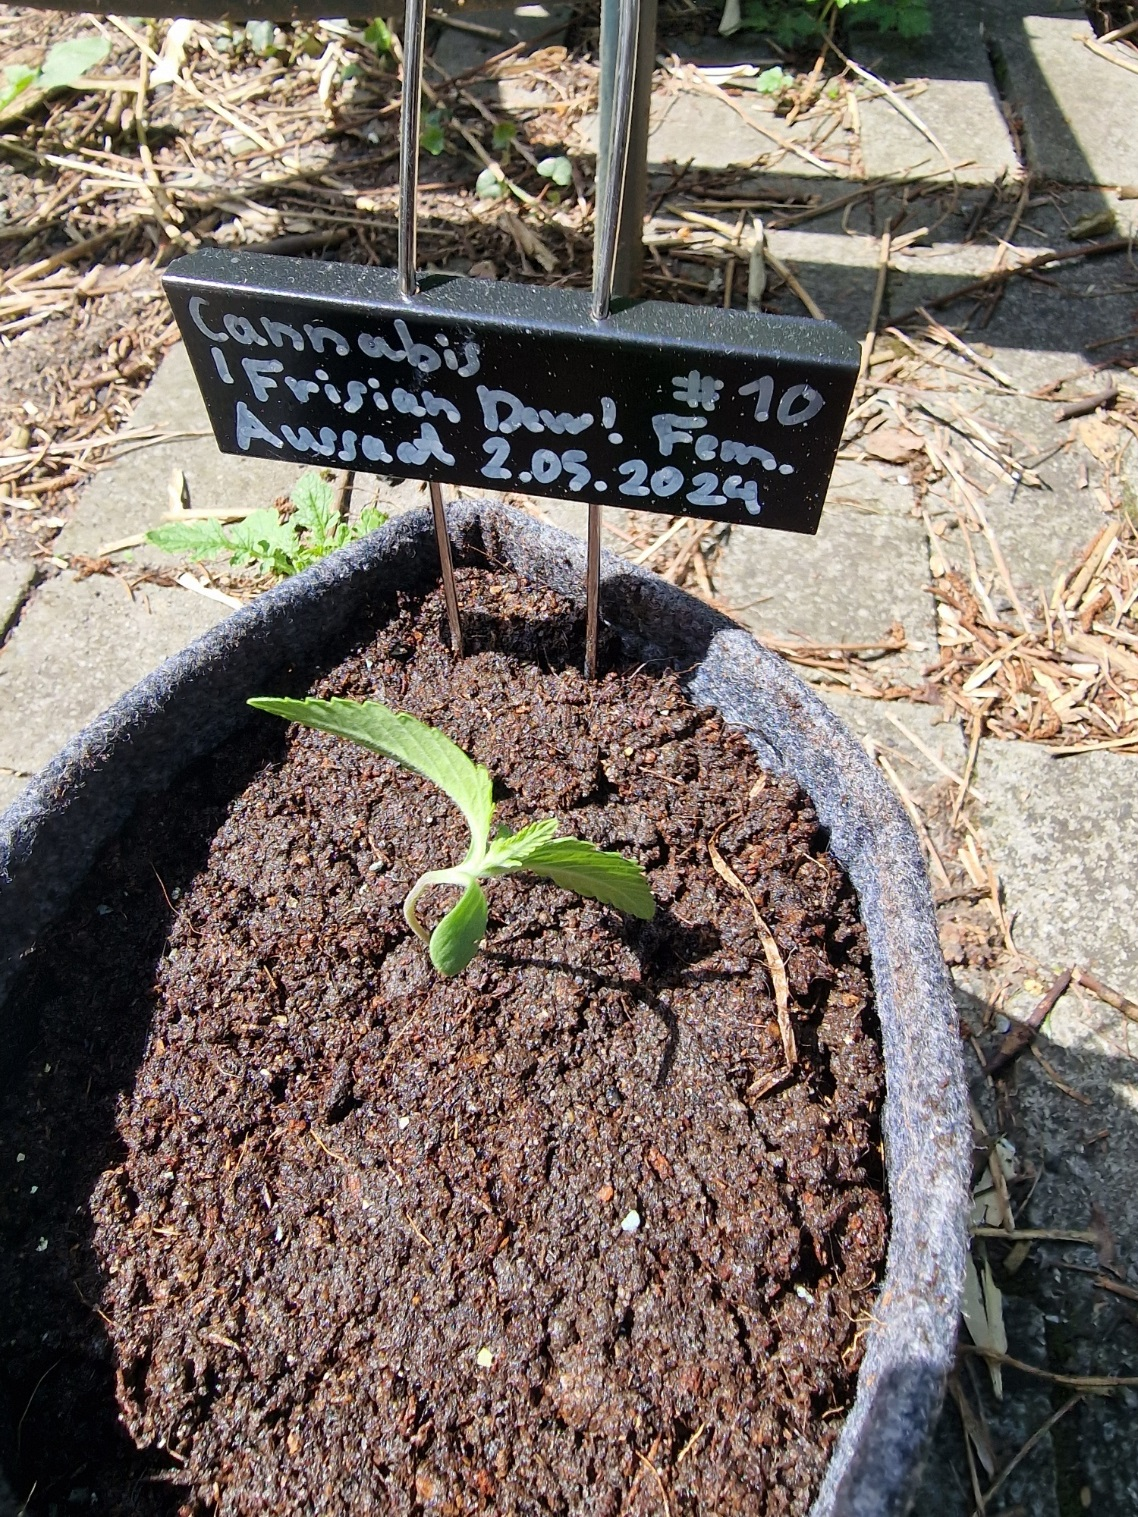
\includegraphics[width=\linewidth]{plant_10_2024-05-13}
        \caption{Plant \# 10}
        \label{fig:plant_10_2024-05-13}
    \end{subfigure}
    \begin{subfigure}[t]{.19\textwidth}
        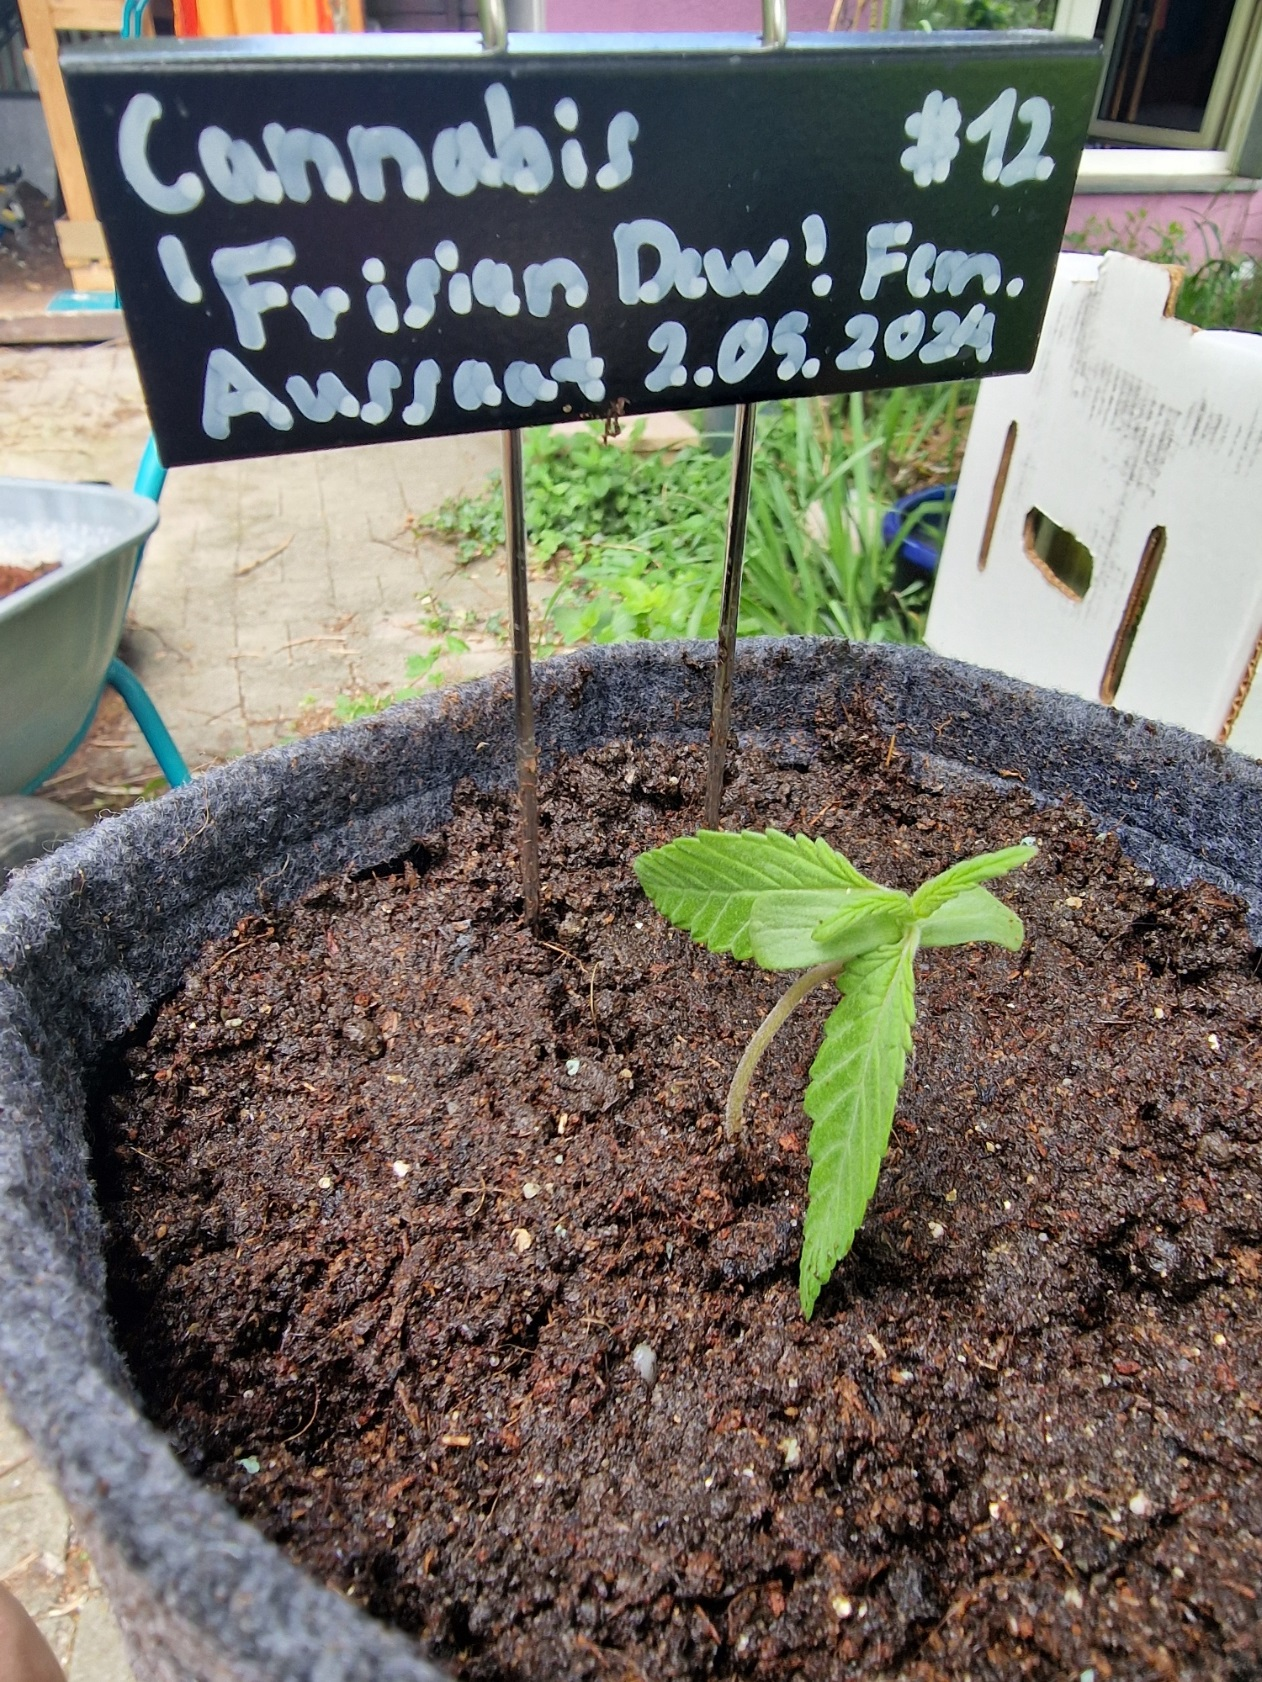
\includegraphics[width=\linewidth]{plant_12_2024-05-13}
        \caption{Plant \# 12}
        \label{fig:plant_12_2024-05-13}
    \end{subfigure}
    \caption[Plants of the control group on May 13]{The plants of the control group on May 13}
    \label{fig:plants_ctrl_2024-05-13}
\end{figure}

\begin{figure}[htbp]
    \begin{subfigure}[t]{.28\textwidth}
        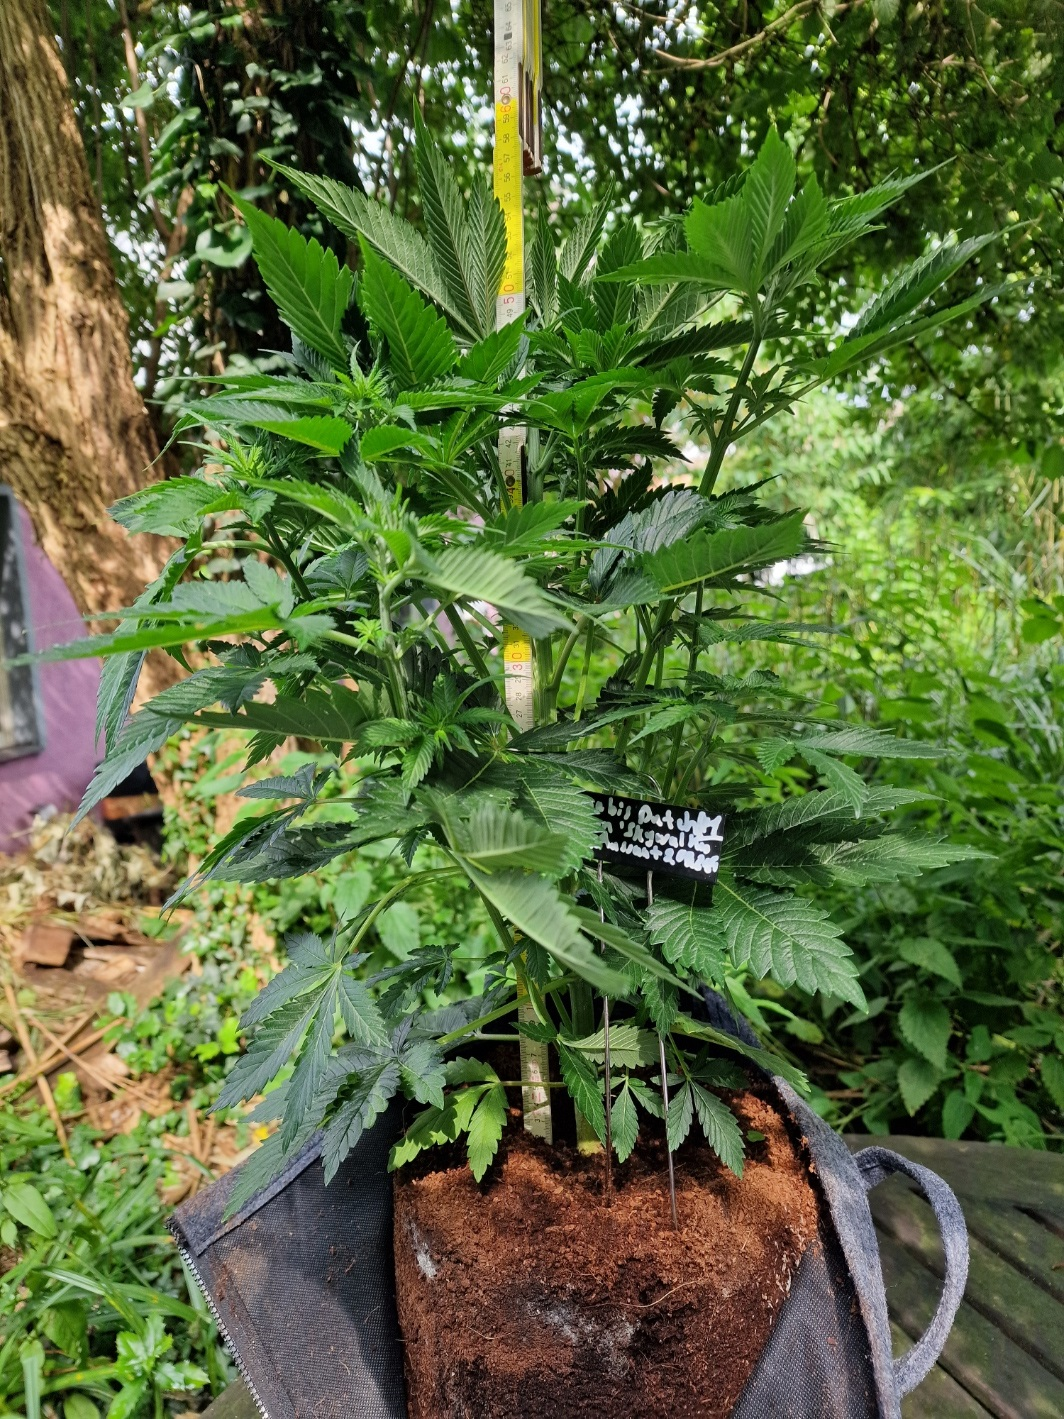
\includegraphics[width=\linewidth]{plant_01_2024-06-17}
        \caption{Plant \# 1}
        \label{fig:plant_01_2024-06-17}
    \end{subfigure}
    \begin{subfigure}[t]{.28\textwidth}
        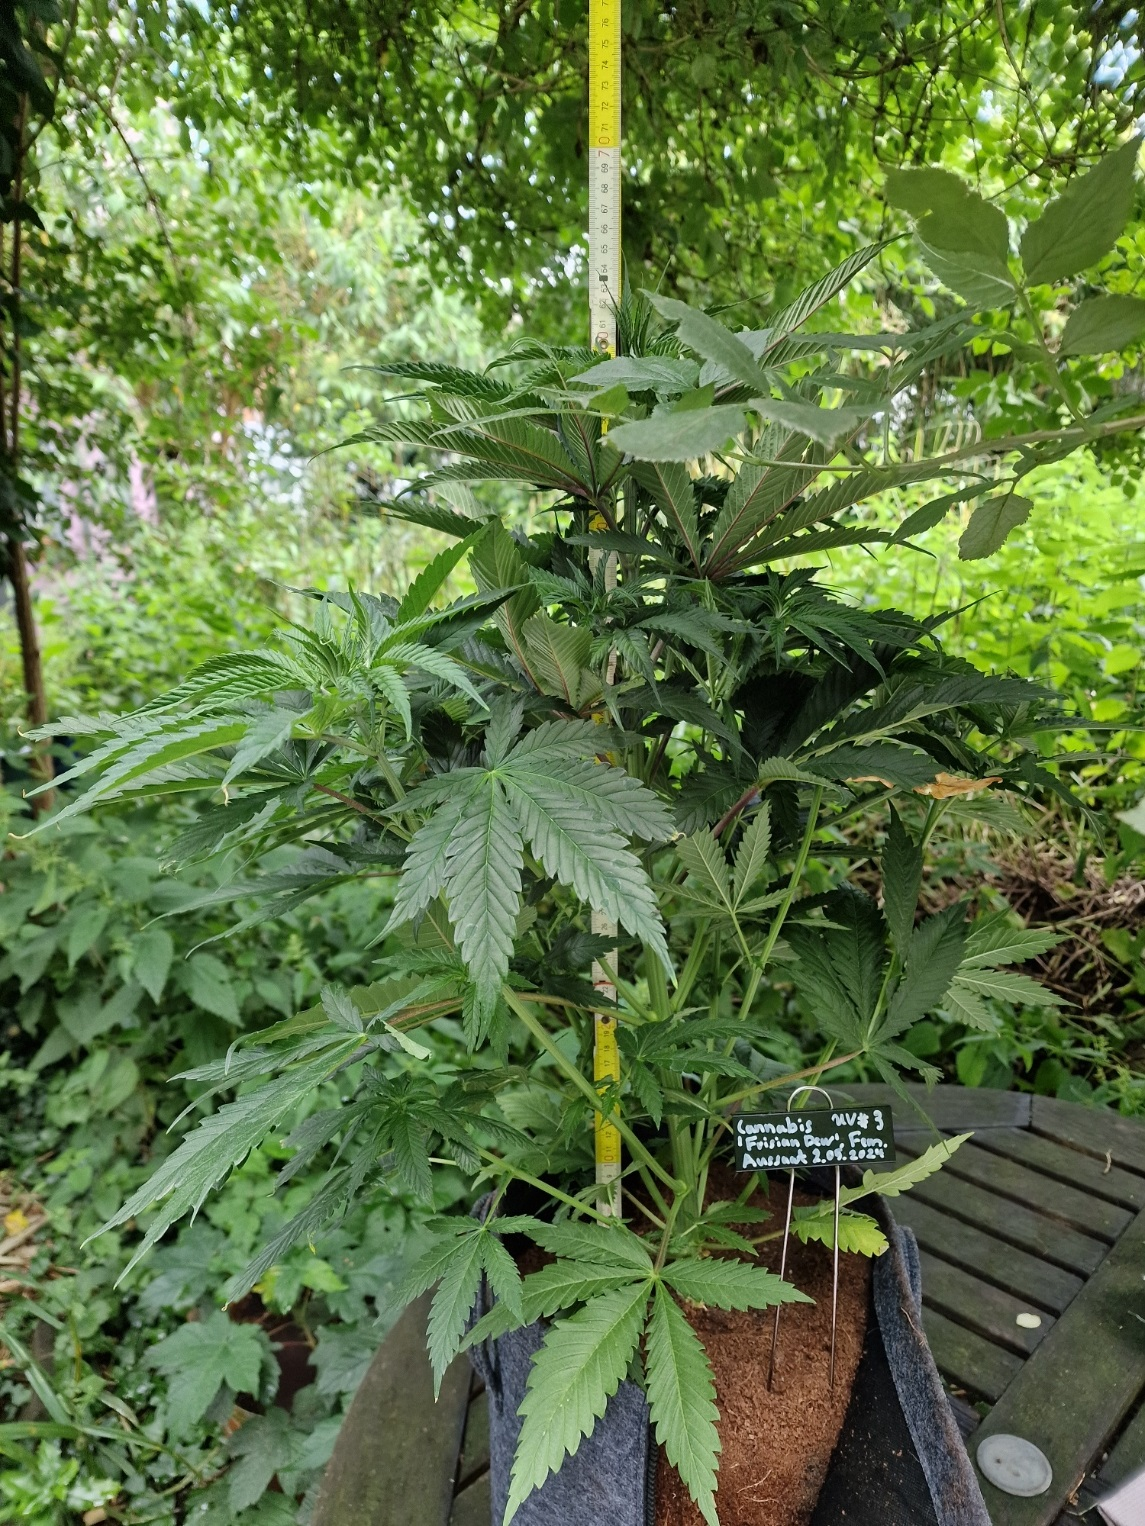
\includegraphics[width=\linewidth]{plant_03_2024-06-17}
        \caption{Plant \# 3}
        \label{fig:plant_03_2024-06-17}
    \end{subfigure}
    \begin{subfigure}[t]{.28\textwidth}
        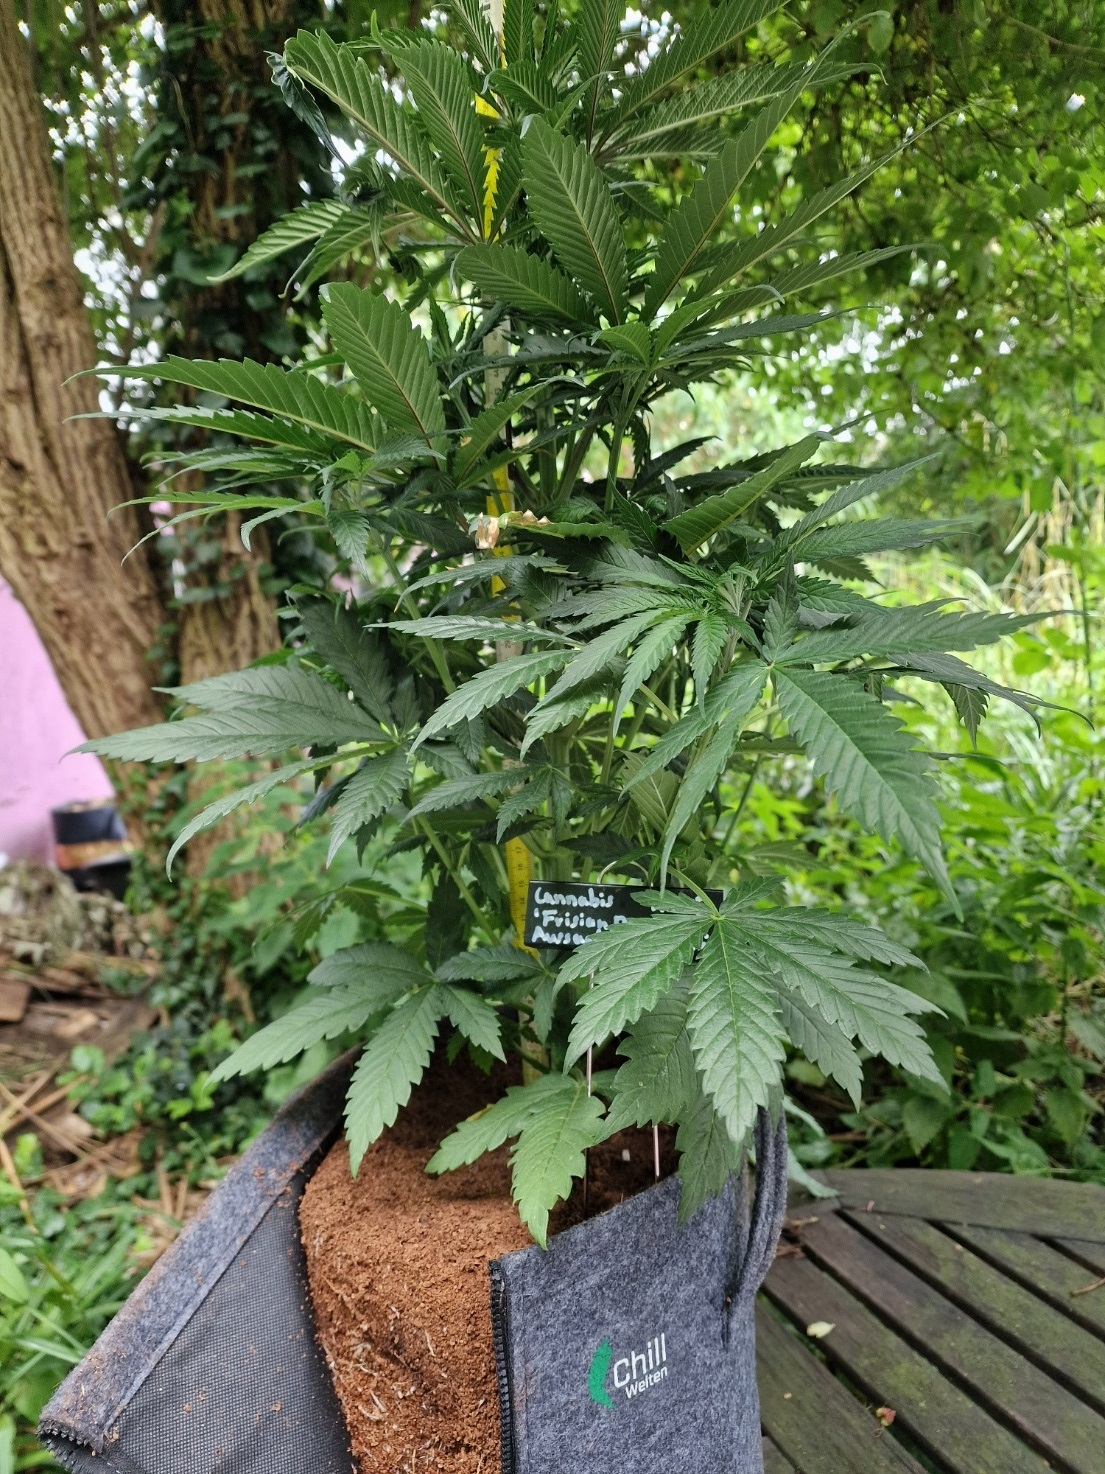
\includegraphics[width=\linewidth]{plant_05_2024-06-17}
        \caption{Plant \# 5}
        \label{fig:plant_05_2024-06-17}
    \end{subfigure}
    \begin{subfigure}[t]{.28\textwidth}
        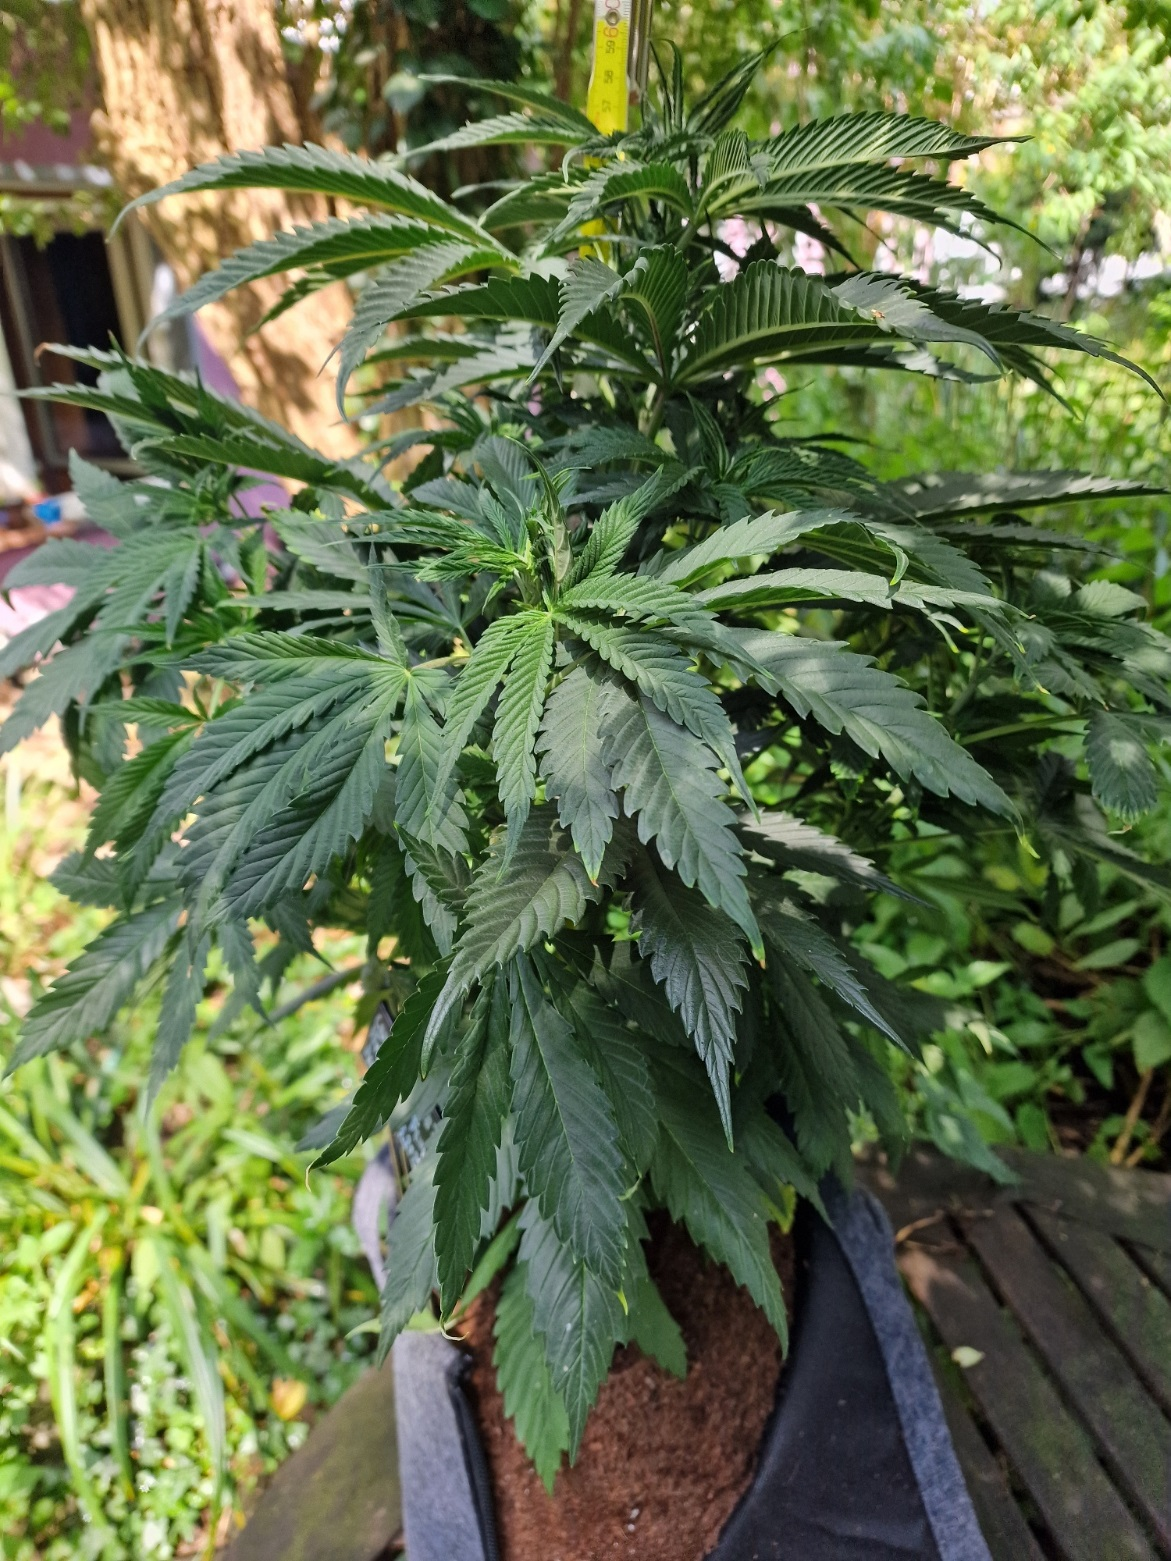
\includegraphics[width=\linewidth]{plant_07_2024-06-17}
        \caption{Plant \# 7}
        \label{fig:plant_07_2024-06-17}
    \end{subfigure}
    \begin{subfigure}[t]{.28\textwidth}
        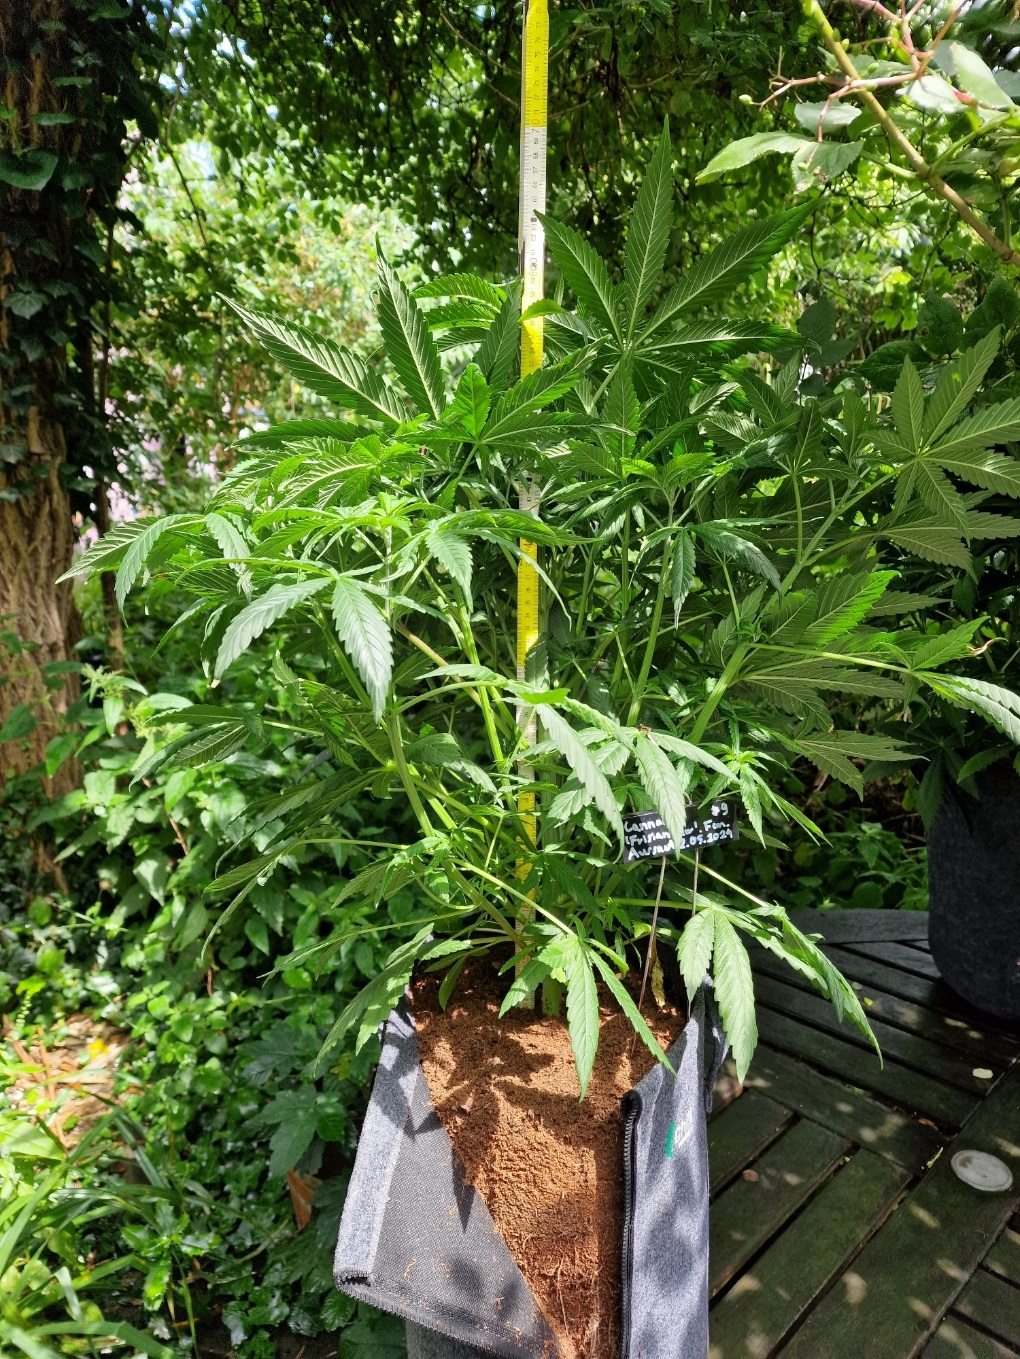
\includegraphics[width=\linewidth]{plant_09_2024-06-17}
        \caption{Plant \# 9}
        \label{fig:plant_09_2024-06-17}
    \end{subfigure}
    \begin{subfigure}[t]{.28\textwidth}
        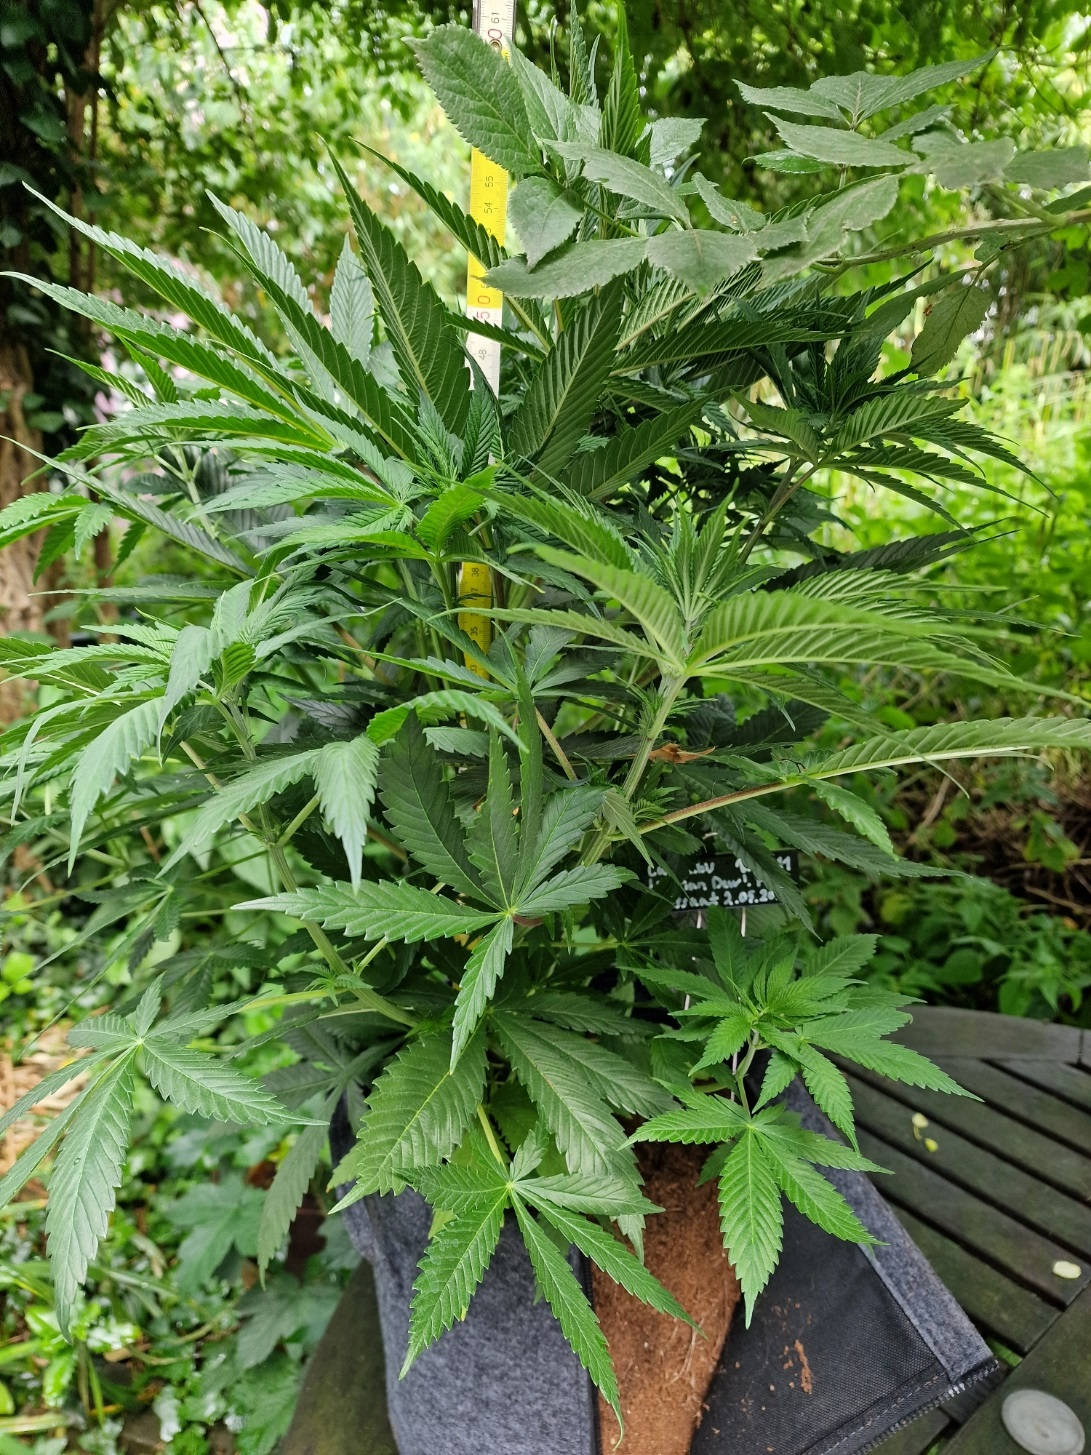
\includegraphics[width=\linewidth]{plant_11_2024-06-17}
        \caption{Plant \# 11}
        \label{fig:plant_11_2024-06-17}
    \end{subfigure}
    \begin{subfigure}[t]{.85\textwidth}
        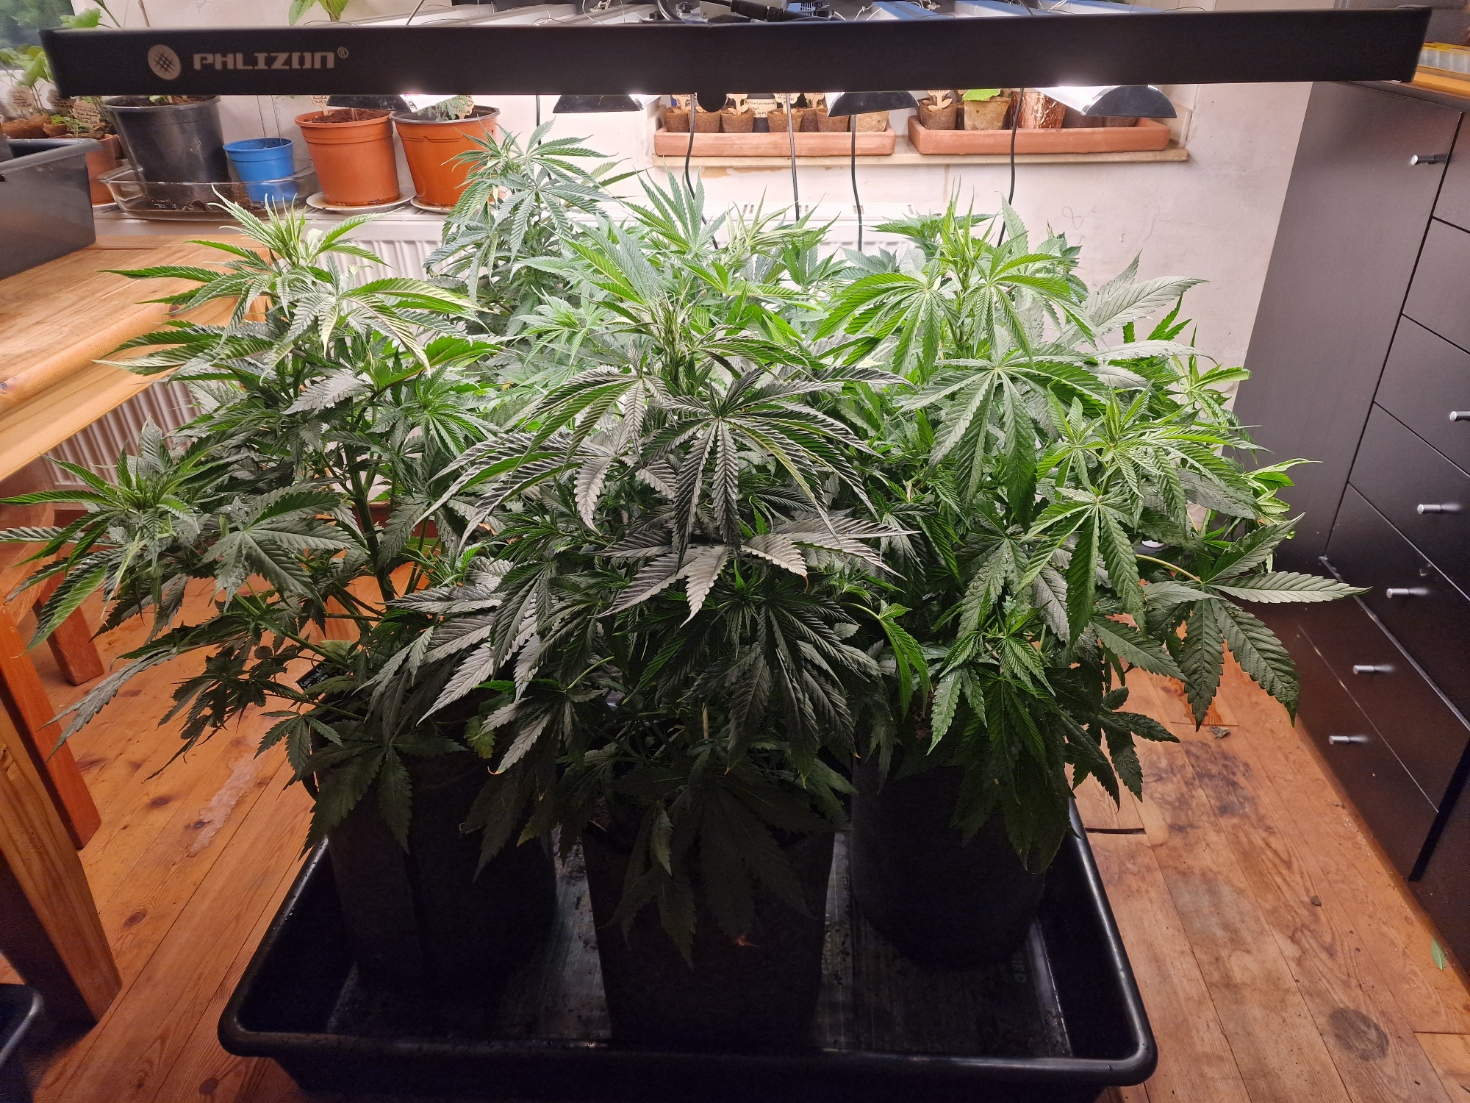
\includegraphics[width=\linewidth]{plant_uv_2024-06-17}
        \caption{All plants of the UV group in their experimental setup under the LED and UV grow lights}
        \label{fig:plant_uv_2024-06-17}
    \end{subfigure}
    \caption[Plants of the UV group on June 17]{The plants treated with UV light on June 17}
    \label{fig:plants_uv_2024-06-17}
\end{figure}

\begin{figure}[htbp]
    \begin{subfigure}[t]{.28\textwidth}
        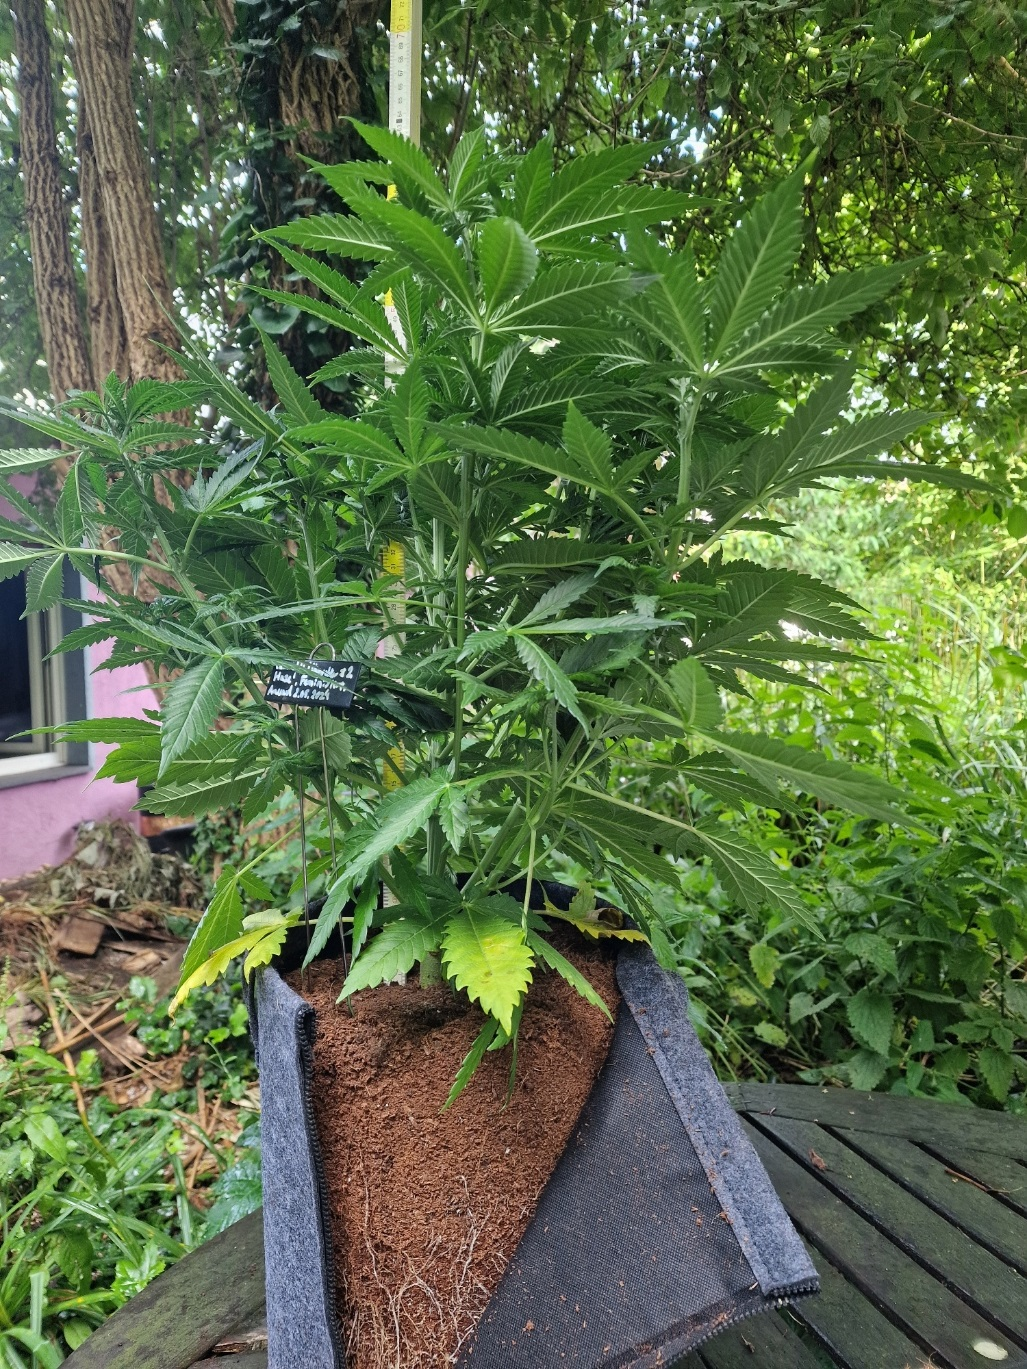
\includegraphics[width=\linewidth]{plant_02_2024-06-17}
        \caption{Plant \# 2}
        \label{fig:plant_02_2024-06-17}
    \end{subfigure}
    \begin{subfigure}[t]{.28\textwidth}
        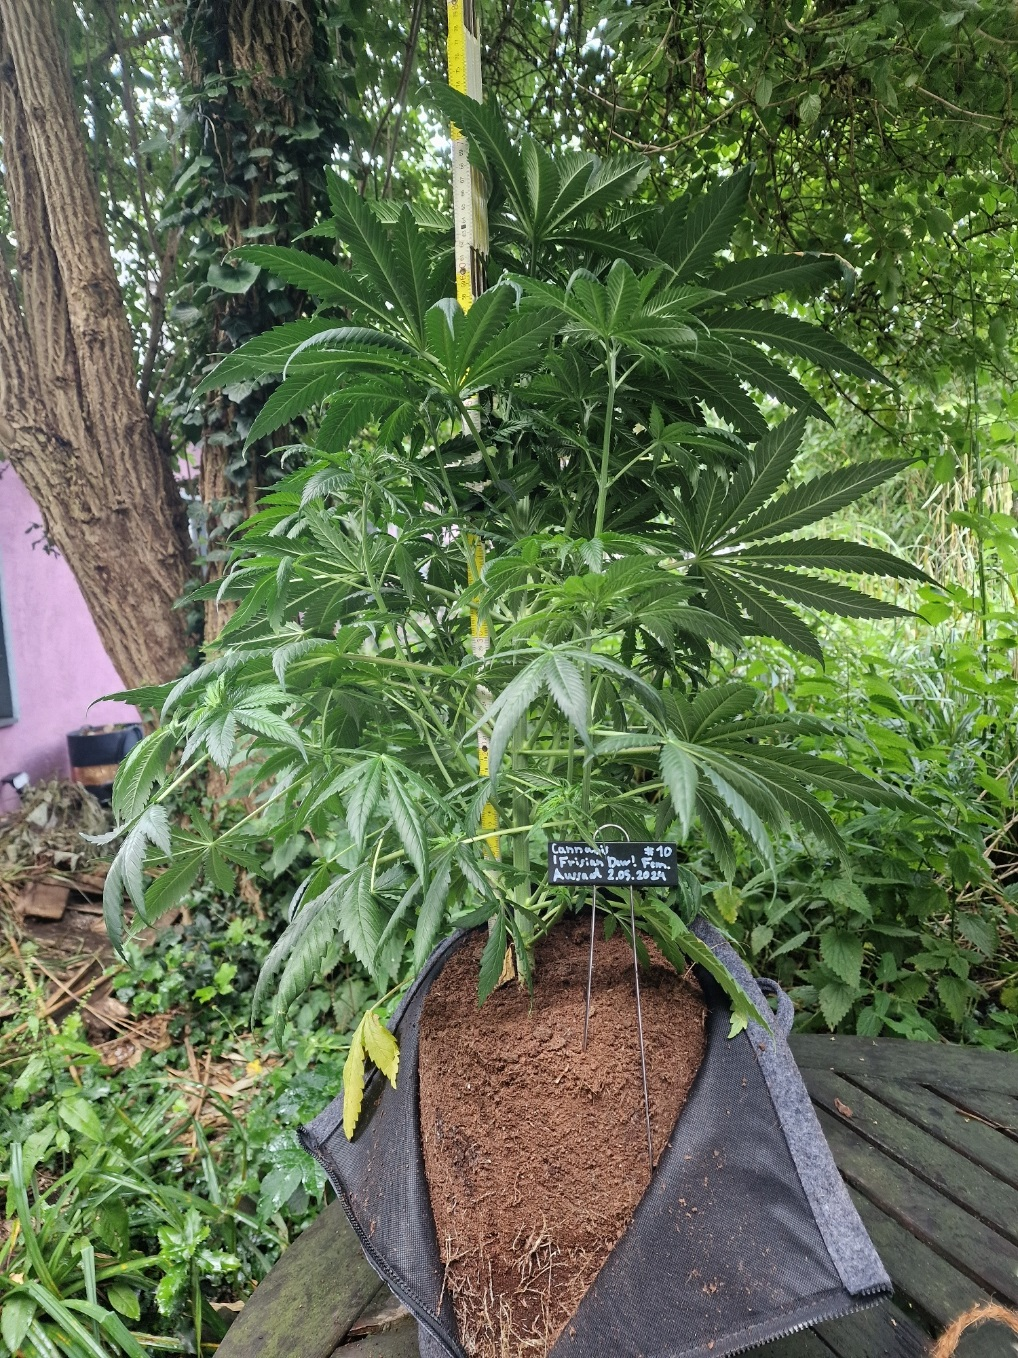
\includegraphics[width=\linewidth]{plant_06_2024-06-17}
        \caption{Plant \# 6}
        \label{fig:plant_06_2024-06-17}
    \end{subfigure}
    \begin{subfigure}[t]{.28\textwidth}
        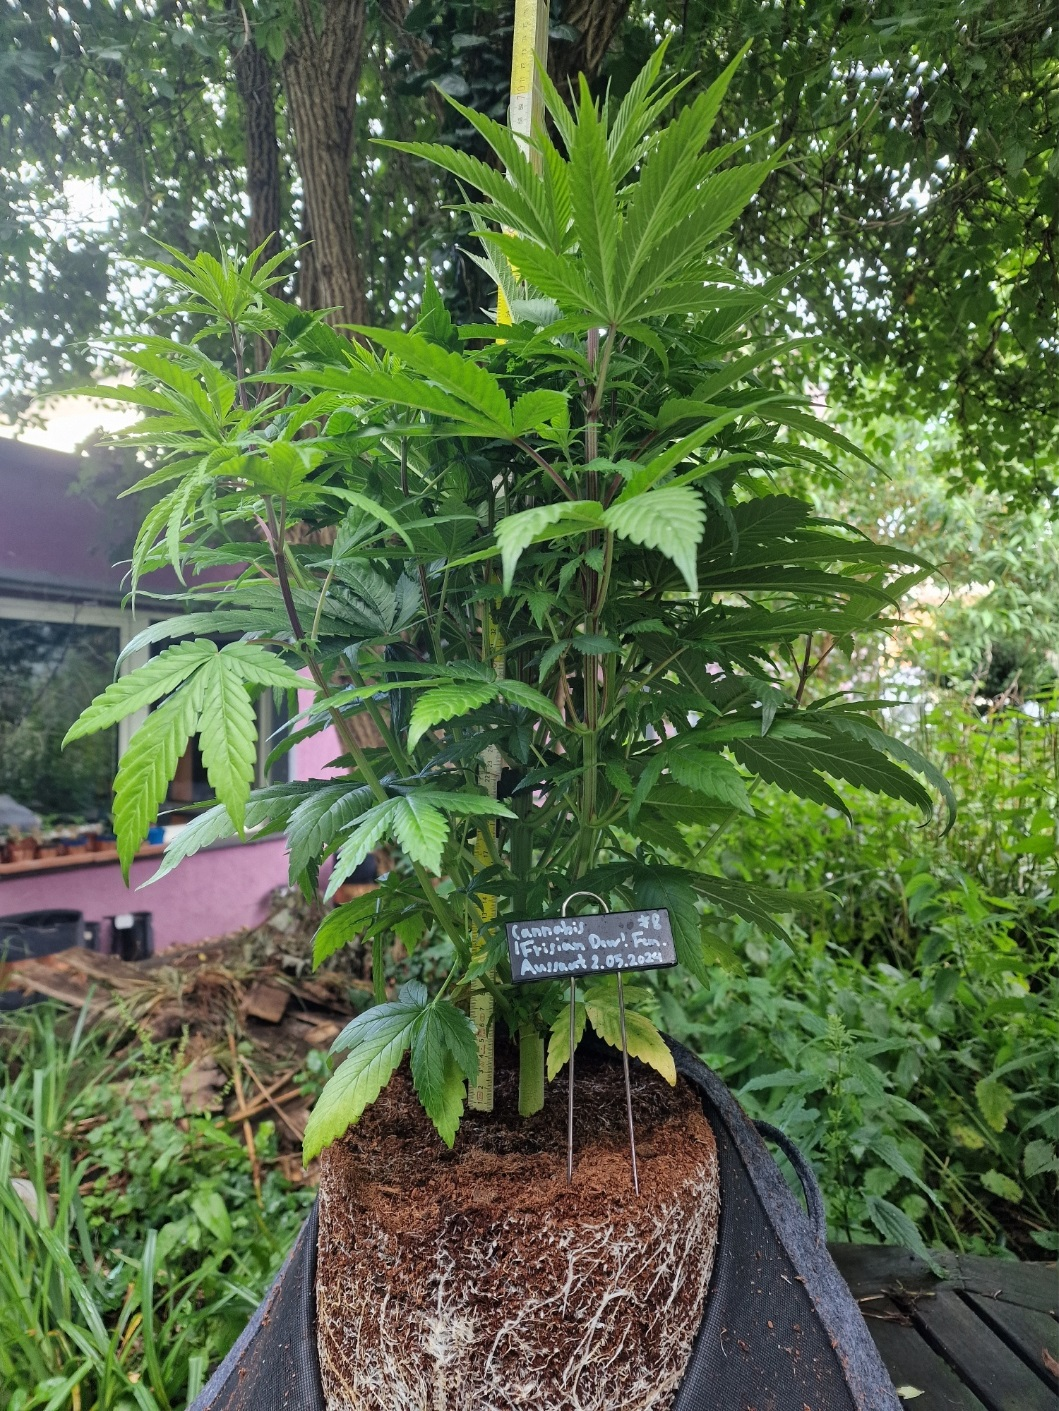
\includegraphics[width=\linewidth]{plant_08_2024-06-17}
        \caption{Plant \# 8}
        \label{fig:plant_08_2024-06-17}
    \end{subfigure}
    \begin{subfigure}[t]{.28\textwidth}
        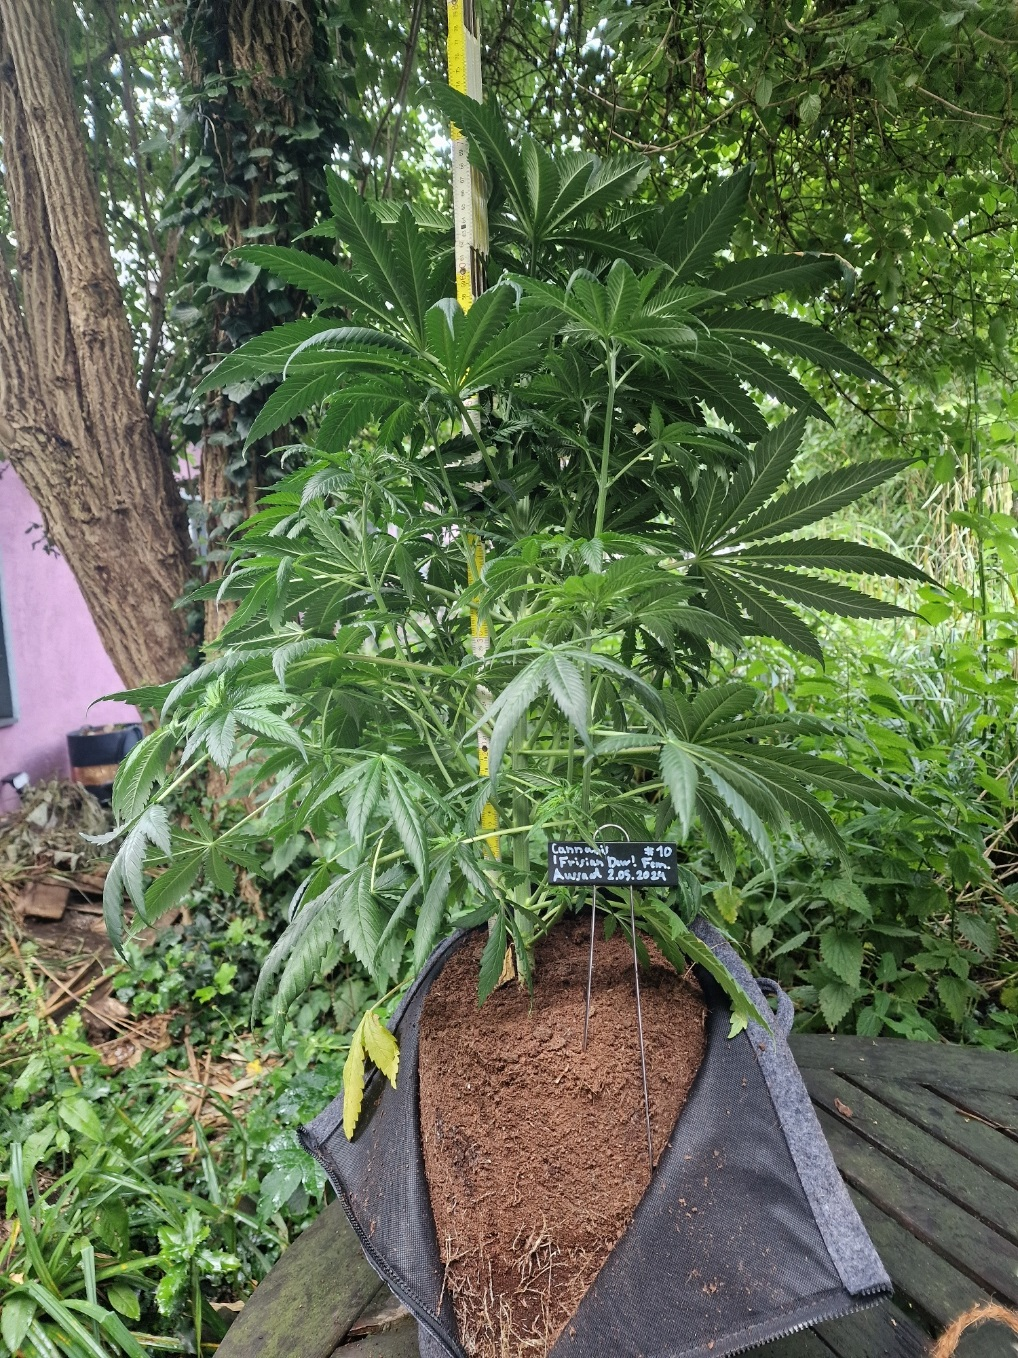
\includegraphics[width=\linewidth]{plant_10_2024-06-17}
        \caption{Plant \# 10}
        \label{fig:plant_10_2024-06-17}
    \end{subfigure}
    \begin{subfigure}[t]{.28\textwidth}
        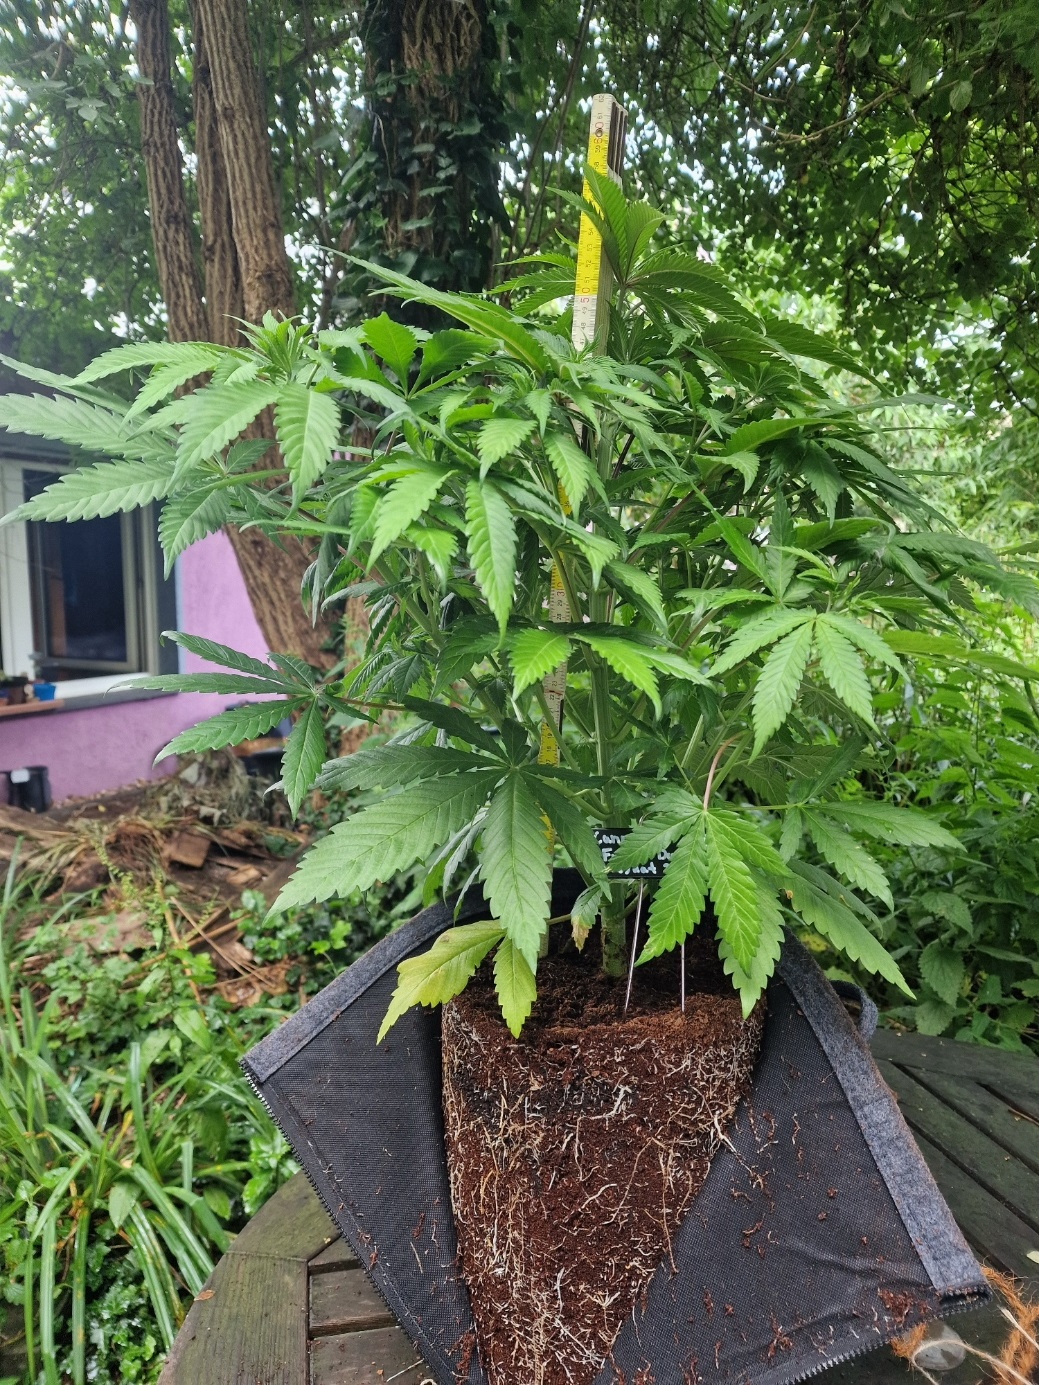
\includegraphics[width=\linewidth]{plant_12_2024-06-17}
        \caption{Plant \# 12}
        \label{fig:plant_12_2024-06-17}
    \end{subfigure}
    \begin{subfigure}[t]{.85\textwidth}
        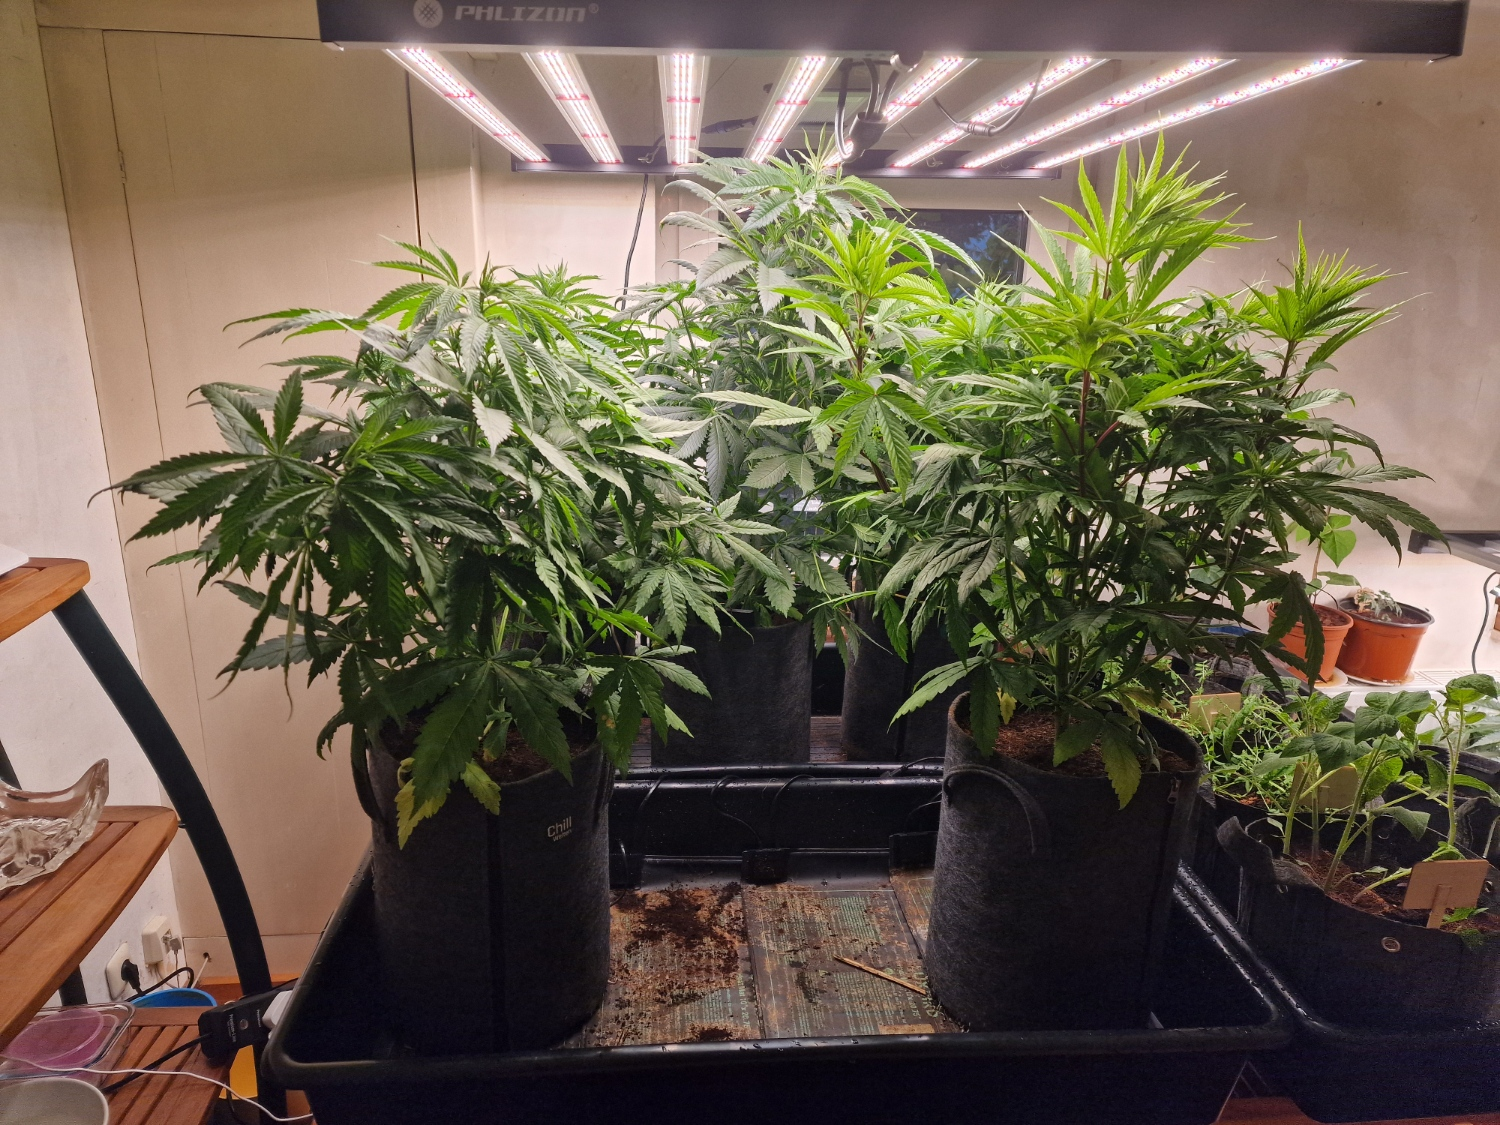
\includegraphics[width=\linewidth]{plant_ctrl_2024-06-17}
        \caption{All plants of the control group in their experimental setup under the LED grow lights}
        \label{fig:plant_ctrl_2024-06-17}
    \end{subfigure}
    \caption[Plants of the control group on June 17]{The plants of the control group on June 17}
    \label{fig:plants_ctrl_2024-06-17}
\end{figure}

\begin{figure}[htbp]
    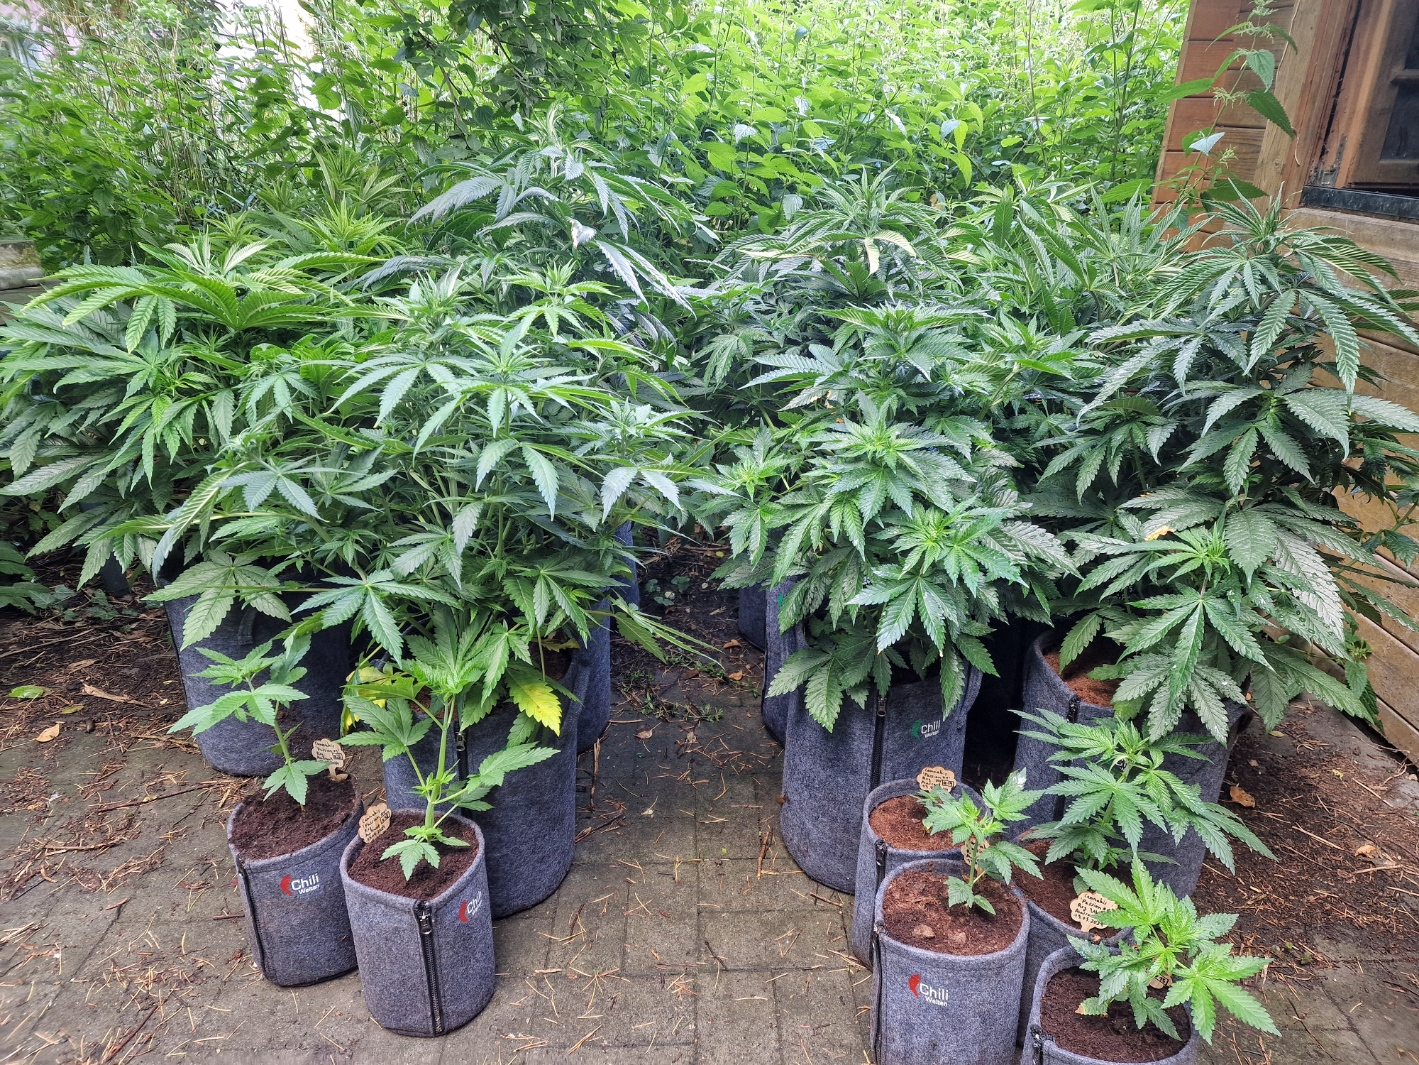
\includegraphics[width=\linewidth]{plant_all_2024-06-17}
    \caption[Plants of both the UV and control groups on June 17]{All plants of both the UV and control groups on June 17. The control group plants are arranged on the left, while the UV group plants are on the right.}
    \label{fig:plant_all_2024-06-17}
\end{figure}